%==============================================================================
% tento soubor pouzijte jako zaklad
% this file should be used as a base for the thesis
% Autoři / Authors: 2008 Michal Bidlo, 2019 Jaroslav Dytrych
% Kontakt pro dotazy a připomínky: sablona@fit.vutbr.cz
% Contact for questions and comments: sablona@fit.vutbr.cz
%==============================================================================
% kodovani: UTF-8 (zmena prikazem iconv, recode nebo cstocs)
% encoding: UTF-8 (you can change it by command iconv, recode or cstocs)
%------------------------------------------------------------------------------
% zpracování / processing: make, make pdf, make clean
%==============================================================================
% Soubory, které je nutné upravit nebo smazat: / Files which have to be edited or deleted:
%   projekt-20-literatura-bibliography.bib - literatura / bibliography
%   projekt-01-kapitoly-chapters.tex - obsah práce / the thesis content
%   projekt-01-kapitoly-chapters-en.tex - obsah práce v angličtině / the thesis content in English
%   projekt-30-prilohy-appendices.tex - přílohy / appendices
%   projekt-30-prilohy-appendices-en.tex - přílohy v angličtině / appendices in English
%==============================================================================
%\documentclass[]{fitthesis} % bez zadání - pro začátek práce, aby nebyl problém s překladem
%\documentclass[english]{fitthesis} % without assignment - for the work start to avoid compilation problem
\documentclass[zadani]{fitthesis} % odevzdani do wisu a/nebo tisk s barevnými odkazy - odkazy jsou barevné
%\documentclass[english,zadani]{fitthesis} % for submission to the IS FIT and/or print with color links - links are color
%\documentclass[zadani,print]{fitthesis} % pro černobílý tisk - odkazy jsou černé
%\documentclass[english,zadani,print]{fitthesis} % for the black and white print - links are black
%\documentclass[zadani,cprint]{fitthesis} % pro barevný tisk - odkazy jsou černé, znak VUT barevný
%\documentclass[english,zadani,cprint]{fitthesis} % for the print - links are black, logo is color
% * Je-li práce psaná v anglickém jazyce, je zapotřebí u třídy použít 
%   parametr english následovně:
%   If thesis is written in English, it is necessary to use 
%   parameter english as follows:
%      \documentclass[english]{fitthesis}
% * Je-li práce psaná ve slovenském jazyce, je zapotřebí u třídy použít 
%   parametr slovak následovně:
%   If the work is written in the Slovak language, it is necessary 
%   to use parameter slovak as follows:
%      \documentclass[slovak]{fitthesis}
% * Je-li práce psaná v anglickém jazyce se slovenským abstraktem apod., 
%   je zapotřebí u třídy použít parametry english a enslovak následovně:
%   If the work is written in English with the Slovak abstract, etc., 
%   it is necessary to use parameters english and enslovak as follows:
%      \documentclass[english,enslovak]{fitthesis}

% Základní balíčky jsou dole v souboru šablony fitthesis.cls
% Basic packages are at the bottom of template file fitthesis.cls
% zde můžeme vložit vlastní balíčky / you can place own packages here

% Kompilace po částech (rychlejší, ale v náhledu nemusí být vše aktuální)
% Compilation piecewise (faster, but not all parts in preview will be up-to-date)
% \usepackage{subfiles}

% Nastavení cesty k obrázkům
% Setting of a path to the pictures
%\graphicspath{{obrazky-figures/}{./obrazky-figures/}}
%\graphicspath{{obrazky-figures/}{../obrazky-figures/}}

%---rm---------------
\renewcommand{\rmdefault}{lmr}%zavede Latin Modern Roman jako rm / set Latin Modern Roman as rm
%---sf---------------
\renewcommand{\sfdefault}{qhv}%zavede TeX Gyre Heros jako sf
%---tt------------
\renewcommand{\ttdefault}{lmtt}% zavede Latin Modern tt jako tt

% vypne funkci šablony, která automaticky nahrazuje uvozovky,
% aby nebyly prováděny nevhodné náhrady v popisech API apod.
% disables function of the template which replaces quotation marks
% to avoid unnecessary replacements in the API descriptions etc.
\csdoublequotesoff



\usepackage{url}


% =======================================================================
% balíček "hyperref" vytváří klikací odkazy v pdf, pokud tedy použijeme pdflatex
% problém je, že balíček hyperref musí být uveden jako poslední, takže nemůže
% být v šabloně
% "hyperref" package create clickable links in pdf if you are using pdflatex.
% Problem is that this package have to be introduced as the last one so it 
% can not be placed in the template file.
\ifWis
\ifx\pdfoutput\undefined % nejedeme pod pdflatexem / we are not using pdflatex
\else
  \usepackage{color}
  \usepackage[unicode,colorlinks,hyperindex,plainpages=false,pdftex]{hyperref}
  \definecolor{hrcolor-ref}{RGB}{223,52,30}
  \definecolor{hrcolor-cite}{HTML}{2F8F00}
  \definecolor{hrcolor-urls}{HTML}{092EAB}
  \hypersetup{
	linkcolor=hrcolor-ref,
	citecolor=hrcolor-cite,
	filecolor=magenta,
	urlcolor=hrcolor-urls
  }
  \def\pdfBorderAttrs{/Border [0 0 0] }  % bez okrajů kolem odkazů / without margins around links
  \pdfcompresslevel=9
\fi
\else % pro tisk budou odkazy, na které se dá klikat, černé / for the print clickable links will be black
\ifx\pdfoutput\undefined % nejedeme pod pdflatexem / we are not using pdflatex
\else
  \usepackage{color}
  \usepackage[unicode,colorlinks,hyperindex,plainpages=false,pdftex,urlcolor=black,linkcolor=black,citecolor=black]{hyperref}
  \definecolor{links}{rgb}{0,0,0}
  \definecolor{anchors}{rgb}{0,0,0}
  \def\AnchorColor{anchors}
  \def\LinkColor{links}
  \def\pdfBorderAttrs{/Border [0 0 0] } % bez okrajů kolem odkazů / without margins around links
  \pdfcompresslevel=9
\fi
\fi
% Řešení problému, kdy klikací odkazy na obrázky vedou za obrázek
% This solves the problems with links which leads after the picture
\usepackage[all]{hypcap}

% Informace o práci/projektu / Information about the thesis
%---------------------------------------------------------------------------
\projectinfo{
  %Prace / Thesis
  project={DP},            %typ práce BP/SP/DP/DR  / thesis type (SP = term project)
  year={2021},             % rok odevzdání / year of submission
  date=\today,             % datum odevzdání / submission date
  %Nazev prace / thesis title
  title.cs={Webová vizualizace dat z~chytrých zařízení v~IoT},  % název práce v češtině či slovenštině (dle zadání) / thesis title in czech language (according to assignment)
  title.en={Web Visualization of Smart Devices Data in IoT
}, % název práce v angličtině / thesis title in english
  %title.length={14.5cm}, % nastavení délky bloku s titulkem pro úpravu zalomení řádku (lze definovat zde nebo níže) / setting the length of a block with a thesis title for adjusting a line break (can be defined here or below)
  %sectitle.length={14.5cm}, % nastavení délky bloku s druhým titulkem pro úpravu zalomení řádku (lze definovat zde nebo níže) / setting the length of a block with a second thesis title for adjusting a line break (can be defined here or below)
  %dectitle.length={14.5cm}, % nastavení délky bloku s titulkem nad prohlášením pro úpravu zalomení řádku (lze definovat zde nebo níže) / setting the length of a block with a thesis title above declaration for adjusting a line break (can be defined here or below)
  %Autor / Author
  author.name={Petr},   % jméno autora / author name
  author.surname={John},   % příjmení autora / author surname 
  author.title.p={Bc.}, % titul před jménem (nepovinné) / title before the name (optional)
  %author.title.a={Ph.D.}, % titul za jménem (nepovinné) / title after the name (optional)
  %Ustav / Department
  department={UIFS}, % doplňte příslušnou zkratku dle ústavu na zadání: UPSY/UIFS/UITS/UPGM / fill in appropriate abbreviation of the department according to assignment: UPSY/UIFS/UITS/UPGM
  % Školitel / supervisor
  supervisor.name={Jiří},   % jméno školitele / supervisor name 
  supervisor.surname={Hynek},   % příjmení školitele / supervisor surname
  supervisor.title.p={Ing.},   %titul před jménem (nepovinné) / title before the name (optional)
  supervisor.title.a={Ph.D.},    %titul za jménem (nepovinné) / title after the name (optional)
  % Klíčová slova / keywords
  keywords.cs={dashboard, vizualizace, IoT, Internet věcí, chytrá zařízení, zobrazení dat, časové série}, % klíčová slova v českém či slovenském jazyce / keywords in czech or slovak language
  keywords.en={dashboard, visualization, IoT, Internet of Things, smart devices, data visualisation, time series}, % klíčová slova v anglickém jazyce / keywords in english
  %keywords.en={Here, individual keywords separated by commas will be written in English.},
  % Abstrakt / Abstract
  abstract.cs={Se stále rostoucím počtem chytrých zařízení roste i potřeba z~nich data ukládat, agregovat a zpracovávat. Získaná data je poté nutné uživateli zpřístupnit efektivním způsobem, díky kterému bude schopný rychle a efektivně reagovat na stav sledovaného zařízení. Tato diplomová práce se zabývá jejich ukládáním a zobrazováním za pomocí dashboardů. Cílem práce bylo vytvořit knihovnu, která bude obsahovat komponenty určené k~zobrazování těchto dat a jednoduchou backendovou aplikaci poskytující API schopnou efektivně ukládat a dotazovat se na data ze senzorů. Knihovna je představena v~jednoduché aplikaci, která využívá vytvořenou backendovou aplikaci. Některé části tohoto řešení byly nasazeny ve firmě Logimic, kde díky nasazení API vrstvy došlo mimo jiné ke~snížení nákladů na provoz databázového systému na 15 \% průměrné ceny dosavadního systému za poslední 2 měsíce. Zbylé části a přístupy jsou nyní postupně integrovány do existujících systémů firmy.}, % abstrakt v českém či slovenském jazyce / abstract in czech or slovak language
  abstract.en={Due to the constant growth in the count of smart devices the need to store, aggregate and process the data effectively rises. The gathered data needs to be displayed effectively to the user, who will be able to react to the current state of the monitored device. This master's thesis deals with storing the data and displaying them using dashboards. The goal of this thesis was the creation of a library composed of components intended for data visualization and a simple API application, that can store and query the data effectively. The library is introduced in a simple application that uses the API application. Some parts of this solution are currently used in the company Logimic, where the costs of the database system reduced to 15 \% of the average cost of the previous database system in the last 2 months. The rest of the solution is currently being integrated into the existing systems of the company.}, % abstrakt v anglickém jazyce / abstract in english
  %abstract.en={An abstract of the work in English will be written in this paragraph.},
  % Prohlášení (u anglicky psané práce anglicky, u slovensky psané práce slovensky) / Declaration (for thesis in english should be in english)
  declaration={Prohlašuji, že jsem tuto diplomovou práci vypracoval samostatně pod vedením pana Ing. Jiřího Hynka, Ph.D. Další informace mi poskytl pan Ing. Michal Valný, Ph.D.
Uvedl jsem všechny literární prameny, publikace a další zdroje, ze kterých jsem čerpal.},
  %declaration={I hereby declare that this Bachelor's thesis was prepared as an original work by the author under the supervision of Mr. X
% The supplementary information was provided by Mr. Y
% I have listed all the literary sources, publications and other sources, which were used during the preparation of this thesis.},
  % Poděkování (nepovinné, nejlépe v jazyce práce) / Acknowledgement (optional, ideally in the language of the thesis)
  acknowledgment={Rád bych poděkoval panu Ing. Jiřímu Hynkovi, Ph.D. a panu Ing. Michalu Valnému, Ph.D. za poskytnutou pomoc a konzultace při tvorbě této práce.},
  %acknowledgment={Here it is possible to express thanks to the supervisor and to the people which provided professional help
%(external submitter, consultant, etc.).},
  % Rozšířený abstrakt (cca 3 normostrany) - lze definovat zde nebo níže / Extended abstract (approximately 3 standard pages) - can be defined here or below
  %extendedabstract={Do tohoto odstavce bude zapsán rozšířený výtah (abstrakt) práce v českém (slovenském) jazyce.},
  %extabstract.odd={true}, % Začít rozšířený abstrakt na liché stránce? / Should extended abstract start on the odd page?
  %faculty={FIT}, % FIT/FEKT/FSI/FA/FCH/FP/FAST/FAVU/USI/DEF
  faculty.cs={Fakulta informačních technologií}, % Fakulta v češtině - pro využití této položky výše zvolte fakultu DEF / Faculty in Czech - for use of this entry select DEF above
  faculty.en={Faculty of Information Technology}, % Fakulta v angličtině - pro využití této položky výše zvolte fakultu DEF / Faculty in English - for use of this entry select DEF above
  department.cs={Ústav matematiky}, % Ústav v češtině - pro využití této položky výše zvolte ústav DEF nebo jej zakomentujte / Department in Czech - for use of this entry select DEF above or comment it out
  department.en={Institute of Mathematics} % Ústav v angličtině - pro využití této položky výše zvolte ústav DEF nebo jej zakomentujte / Department in English - for use of this entry select DEF above or comment it out
}

% Rozšířený abstrakt (cca 3 normostrany) - lze definovat zde nebo výše / Extended abstract (approximately 3 standard pages) - can be defined here or above
%\extendedabstract{Do tohoto odstavce bude zapsán výtah (abstrakt) práce v českém (slovenském) jazyce.}
% Začít rozšířený abstrakt na liché stránce? / Should extended abstract start on the odd page?
%\extabstractodd{true}

% nastavení délky bloku s titulkem pro úpravu zalomení řádku - lze definovat zde nebo výše / setting the length of a block with a thesis title for adjusting a line break - can be defined here or above
%\titlelength{14.5cm}
% nastavení délky bloku s druhým titulkem pro úpravu zalomení řádku - lze definovat zde nebo výše / setting the length of a block with a second thesis title for adjusting a line break - can be defined here or above
%\sectitlelength{14.5cm}
% nastavení délky bloku s titulkem nad prohlášením pro úpravu zalomení řádku - lze definovat zde nebo výše / setting the length of a block with a thesis title above declaration for adjusting a line break - can be defined here or above
%\dectitlelength{14.5cm}

% řeší první/poslední řádek odstavce na předchozí/následující stránce
% solves first/last row of the paragraph on the previous/next page
\clubpenalty=10000
\widowpenalty=10000

% checklist
\newlist{checklist}{itemize}{1}
\setlist[checklist]{label=$\square$}

% Nechcete-li, aby se u oboustranného tisku roztahovaly mezery pro zaplnění stránky, odkomentujte následující řádek / If you do not want enlarged spacing for filling of the pages in case of duplex printing, uncomment the following line
% \raggedbottom

\begin{document}
  % Vysazeni titulnich stran / Typesetting of the title pages
  % ----------------------------------------------
  \maketitle
  % Obsah
  % ----------------------------------------------
  \setlength{\parskip}{0pt}

  {\hypersetup{hidelinks}\tableofcontents}
  
  % Seznam obrazku a tabulek (pokud prace obsahuje velke mnozstvi obrazku, tak se to hodi)
  % List of figures and list of tables (if the thesis contains a lot of pictures, it is good)
  \ifczech
    \renewcommand\listfigurename{Seznam obrázků}
  \fi
  \ifslovak
    \renewcommand\listfigurename{Zoznam obrázkov}
  \fi
  % {\hypersetup{hidelinks}\listoffigures}
  
  \ifczech
    \renewcommand\listtablename{Seznam tabulek}
  \fi
  \ifslovak
    \renewcommand\listtablename{Zoznam tabuliek}
  \fi
  % {\hypersetup{hidelinks}\listoftables}

  \ifODSAZ
    \setlength{\parskip}{0.5\bigskipamount}
  \else
    \setlength{\parskip}{0pt}
  \fi

  % vynechani stranky v oboustrannem rezimu
  % Skip the page in the two-sided mode
  \iftwoside
    \cleardoublepage
  \fi

  % Text prace / Thesis text
  % ----------------------------------------------
  \ifenglish
    \input{projekt-01-kapitoly-chapters-en}
  \else
    \chapter{Úvod}
Se stále rostoucím počtem chytrých zařízení roste i množství dat, která je zapotřebí zobrazit. Díky tomuto nárůstu se neustále zvyšují nároky na použité vizualizace, které musí svému uživateli zobrazit data takovým způsobem, aby mohl rychle a aktivně reagovat na zobrazené informace. V dnešní době bohužel nejsou časté platformy, které by poskytovaly možnost tohoto zobrazení pokud možno pro uživatele jednoduchým a interaktivním způsobem.

Příkladem oblasti, kde je této platformy zapotřebí může být vytápění, kde v minulosti každé domácnosti stačil klasický kotel na tuhá paliva v dnešní době má většina z nich kotel na jiná paliva (plyn, elektrický) nebo automatický kotel na tuhá paliva. Mnoho z těchto zařízení poskytuje možnost nastavit způsob vytápění bezdrátově za pomocí mobilní aplikace z pohodlí obývákového gauče. Tímto se řadí mezi takzvané IoT zařízení, tedy zařízení, které plní nějakou specifickou funkci (například vytápění), je připojeno k internetu a dokáže přes něj komunikovat s dalším zařízením ve stejné síti. Počet a zájem o tyto zařízení neustále roste, nejsou zaměřené pouze na vytápění ale také na další aspekty našeho každodenního života. Příkladem dalších zařízení může být nositelná elektronika jako chytré hodinky nebo fitness náramky, solární panely a to jak fotovoltaické tak panely pro ohřev vody, automatické brány, 3d tiskárny a další. Výrobci těchto zařízení často poskytují i zmíněné aplikace k jejich ovládání, ale ty často zobrazují pouze část aktuálního stavu.

Mnoho IoT zařízení dovoluje získávat přes internet svůj stav a tím zpřístupňuje možnost zkontrolování správné funkce nebo stavu zařízení na dálku. Otázkou ale zůstává jak data z jednotlivých zařízení získávat, ukládat a zobrazovat uživateli tak, aby je byl schopen bezpracně a bezstarostně vyhodnotit.

Tato situace se ale netýká pouze osobních zařízení a domácích spotřebičů ale také z velké části průmyslu, který se postupem času stále více automatizuje a operace, které dříve bylo nutné vykonávat ruční prací jsou vykonávány strojově. Tyto stroje ale nejsou bezchybné a je potřeba je monitorovat. Část monitorování je také možné automatizovat, ale nakonec je vždy zapotřebí lidská kontrola. 

Tento úkol se na první pohled může jevit jako jednoduchý, bohužel každé zařízení často vyžaduje unikátní způsob zobrazení a to nejen například kvůli povaze daných dat, ale také například kvůli tomu, že nás nezajímají pouze holá data ale například extrémy hodnot nebo relace mezi hodnotami samotnými. Práce s daty také přináší problémy se kterými je nutné se vypořádat. Data mohou obsahovat špatné nebo zkreslené záznamy, nebo jich může být příliš velké množství pro smysluplné zpracování. Problematikou efektivního zobrazování a ukládání se zabývá poměrně velké množství firem. Jednou z nich je i firma Logimic, se kterou jsem při řešení této diplomové práce spolupracovalo.

Tato diplomová práce se snaží vyřešit některé ze zmíněných problémů a to hlavně způsoby, jakými je možné data efektivně zobrazit uživateli v takovém formátu, aby pro něj byla jednoduše interpretovatelná a efektivní způsoby uložení velkého množství dat ze senzorů. Za těmito účely budou vytvořeny dvě aplikace. První aplikace založená na aplikačním rámci Angular a bude sloužit k zobrazení dat. Druhá aplikace bude sloužit k demonstraci efektivních způsobů ukládání potřebných dat.

Kapitola \ref{chapter_iot} poskytuje přesnější popis Internetu věcí, přehled senzorů, které je v této oblasti možné využít a způsoby komunikace. Způsoby efektivního uložení dat z IoT zařízení jsou obsaženy v kapitole \ref{chapter_db}. Kapitola \ref{chapter_dashboard} obsahuje popis pohledů dashboard, vizualizace v nich použitelné, popis KPI a přístupy k detekci anomálií. Kapitola \ref{chapter_visualisation} obsahuje popis technologií, které je možné využít k vytváření uživatelských rozhraní. V kapitole \ref{chapter_analysis} je obsažena analýza aktuálního stavu ve firmě Logimic. Návrh řešení je obsažen v kapitole \ref{chapter_desing}. V následující kapitole \ref{chapter_implemenatation} je obsažena implementace tohoto řešení následovaná kapitolou \ref{chapter_testing} obsahující testování vytvořeného řešení.

%První \ref{chapter_iot} kapitola poskytuje přesnější popis Internetu věcí, přehled senzorů, ktere je v této oblasti možné využít a způsoby komunikace, které využívají a přehled technologií, které je možné použít pro efektivní uložení dat ze senzorů a rozdíly mezi nimi. V druhé kapitole jsou popsány způsoby návrhů dashboardů a aspekty lidského vnímání, které je nutné při jejich návrhu vzít v potaz. Ve třetí kapitole je obsažen přehled technologií, které jsou v současné době používány k implementování dashboarů.Ve čtvrté kapitole je obsažena analýza aktuálního stavu ve firmě Logimic a analýza požadavků na vizualizaci dat získaných ze senzorů. V páté kapitole je obsažen návrh pohledů a způsobu jejich integrace do informačního systému a způsoby uložení. V šesté kapitole je obsažen popis vlastní implementace pohledů a informačního systému včetně popisu vybraných technologií a důvodů k jejich výběru. V poslední části je obsažen popis metodiky testování a výsledky tohoto testování.
\chapter{Internet věcí}
\label{chapter_iot}
Internet věcí, IoT z anglického Internet of Things, je možné obecně definovat jako věci nebo objekty, které jsou připojeny nějakou technologií k internetu, nebo k dalším IoT zařízením. Zájem o zařízení tohoto typu rychle roste, nejen v soukromém prostoru, ale i v průmyslu. Důkazem může být například i to, že odhadovaný počet IoT zařízení v roce 2021 podle některých zdrojů 10 -- 12 miliard zařízení \cite{iotAnalytics_2021, holst_2021} a stále se odhaduje další nárůst. Z praktického pohledu musí být každému zařízení přidělen unikátní identifikátor (UID) a IP adresa, aby s ním bylo možné komunikovat přes některou z vybraných technologií, mezi které patří například WiFi nebo tradiční ethernet.

Kromě tradičního chápání IoT existují ještě další způsoby \cite{greengard2015internet}, které tuto problematiku popisují jiným způsobem. Některé zdroje používají pojem “propojené zařízení” pro jakákoli zařízení, která jsou spolu spojena. Tyto zařízení nutně nemusí být připojena do internetu, ale stále častěji se k němu připojují. Další zdroje používají pouze podkategorii IoT, kterou nazývají Industriální internet. Tento Industriální internet se specializuje pouze na zařízení, která je možné použít v průmyslu a často dělí zařízení v něm podle toho, jestli komunikují s uživatelem nebo pouze s ostatními zařízeními v síti. Posledním typem, který stojí za zmínění je takzvaný internet všeho, Internet of Everything, který se více vrací k původní definici IoT a byl navržen firmou Cisco. Tato práce používá původní definici IoT a to z jednoduchého důvodu. Ostatní definice buď vychází z této definice nebo se zaměřují na její podmnožinu.

\section{Typy sensorů}
Ve světe IoT se nachází velký počet typů sensorů a způsobů, jak je možné na ně nahlížet při jejich dělení. Díky těmto dělením je často možné vybrat odpovídající způsob nejen uložení ale i zobrazení uživateli. Například data z GPS je nutné uživateli zobrazit jiným způsobem než naměřenou teplotu za poslední hodinu.

Prvním z možných způsobů dělení je dělení na základě měřené fyzikální veličiny \cite{8862778}, například na světelné senzory, které měří intenzitu světla, senzory teploty, vlhkosti, vzdálenosti a další. Toto rozdělení je ale zaměřené na měřenou veličinu, kterou je možné reprezentovat číselně a kvůli tomu nám nerozdělí velkou skupinu senzorů.

Druhým způsobem je dělení na základě toho, k čemu jsou jejich data využita při řešení různých problémů, například na základě toho, jak je možné je využít pro zlepšení využití elektrické energie \cite{7946568}, kde senzory rozdělují následovně:
\begin{itemize}
\item senzory obsazenosti -- řeší, zda-li je daný objekt aktuálně obsazený či obývaný, například pomocí pohybových senzorů, senzorů reagujících na vibrace a dalších,
\item senzory prostředí -- měří podmínky, které jsou aktuálně v daném objektu, tedy například teplotu, kvalitu vzdudu, množství CO\textsubscript{2} za pomocí senzorů k měření těchto fyzikálních veličin,
\item monitory napájení -- specializované senzory, které měří aktuální využití elektrické energie v daném objektu za pomocí speciálních senzorů například od firmy Wattvision,
\item ostatní senzory -- jakékoli další senzory, které je možné využít k zlepšení využití elektrické energie jako například elektronické zásuvky, chytré žárovky a další.
\end{itemize}

Třetím způsobem rozdělení je rozdělení podle způsob komunikace, kterou využívají dané zařízení pro přenos dat \cite{8079928}. K tomuto účelu se většinou používají bezdrátové technologie a to hlavně z toho důvodu, že přivedení klasického internetového spojení může být nepraktické, například protože je zařízení na nedostupném místě, nebo je pohyblivé. 

Bezdrátové technologie se často dělí podle dosahu technologie na nízkonapěťové rozlehlé sítě z anglického Low Power Wide Area Network a sítě krátkého dosahu. Nejznámějšími zástupci nízko napěťových rozlehlých sítí jsou následující technologie:

\begin{itemize}
\item SigFox -- technologie vhodná pro přenášení malého množství dat mezi IoT zařízeními do maximální vzdálenosti 50 kilometrů za pomocí velmi krátkých vln.
\item Celulární sítě -- tradiční technologie většinou používaná pouze k připojení telefonních zařízeních, ale je možné je využít i k připojení IoT zařízení. Oproti technologii SigFox poskytují celulární sítě dostupnost na větší vzdálenosti, ale jsou více vhodné k ovládání uživatelem než k přenosu dat mezi zařízeními.
\end{itemize}

Pro komunikaci v malých sítích, nebo sítích, kde je zapotřebí přenášet velké množství dat mezi zařízeními, je častější využití sítí s kratším dosahem. K nejvýznamnějším z těchto technologií patří následující technologie:

\begin{itemize}
\item 6LoWPAN -- technologie využívající protokol IPv6 pro přenos dat přes bezdrátové osobní sítě s nízkou spotřebou. Jak již napovídá název tato technologie využívá standardizovaný protokol IPv6 a je tedy možné jednoduše komunikovat s tradičními zařízeními. Narozdíl od tradiční WiFi se tato technologie zaměřuje na nízkou spotřebu, cenu, dosah a cenu \cite{rfc4919}.

\item Bluetooth -- technologie pro přenos dat v osobních sítích, kvůli nedostatkům z pohledu použití v IoT, konkrétně vysoké spotřeby, pomalé inicializace a omezeného počtu zařízení je nyní nahrazován technologií BLE, bluetooth low energy, která není s původní technologií kompatibilní, ale snaží se odstranit její nevýhody.
\item RFID -- technologie založená na unikátních ID tagů, které je možné číst použitím rádiových antén, často využívané pro kontrolu přístupu, celní systémy nebo logistice \cite{10.1007/11687238_36}. V dnešní době je spíše používaná varianta takzvaného pasivního RFID, která nepotřebuje napájení tagu.
\item NFC -- technologie NFC je založená na technologii RFID a je také určena na přenos dat na velmi krátké vzdálenosti. Narozdíl od RFID poskytuje možnost pouze pasivního tagu, každé spojení je omezeno pouze na dvě zařízení. Technologie je často využívána pro platby mobilním telefonem \cite{coskun2011near}.
\end{itemize}

Kromě těchto rozdělení existují i zařízení, které na první pohled nejsou tradičními senzory a často je tak nechápeme. Příkladem mohou být například kamerové systémy, které mohou nejen plnit funkce jiných senzorů. Záznam z kamery může být například využít k detekci pohybu, ale také poskytují unikátní možnosti. Příkladem těchto možností u již zmíněných kamerových systémů může být například detekce hustoty provozu a přizpůsobení časování semaforů za účelem zvýšení plynulosti provozu, nebo automatické vyhledávání hledaných osob.

Všechny tyto senzory ale mají společné vlastnosti. Hlavní podobnou vlastností je fakt, že senzory sledují závislost fyzické veličiny nebo stavu v aktuálním čase. Díky tomu se dají tato data chápat jako takzvané časové řady nebo časové série (anglicky \textit{time series}). Při práci s nimi často rozdělujeme časové série na série událostí a měření. Typičtější jsou měření, kdy je ve stanoveném čase měřena hodnota senzoru. Tento přístup nám dovoluje zachytávat měřenou veličinu, která se postupně a neustále vyvíjí, jako například teplota. Na druhou stranu série událostí vyjadřují pouze diskrétní změny stavu, kdy není zapotřebí několikrát ukládat stejnou hodnotu, ale jsou důležité pouze její změny.

Tato diplomová práce se specializuje na jakékoli senzory, jejiž hodnoty je možné prakticky reprezentovat číselně, nebo za pomocí textových řetězců obou typů časových sérií. Ostatní senzory vyžadují radikálně odlišné přístupy tak, jak je tomu například u již zmíněných kamerových systémů.

\section{Existující cloudová řešení} %TODO fix name
Chytrá zařízení je často velmi praktické spojovat do větších sítí. Jednotlivé senzory totiž nemusí poskytovat všechny potřebné informace a centralizace získaných informací sníží požadavky na koncová zařízení. Za tímto účelem je nutné zvolit strategii použitou ke vzájemnému propojení zařízení, kdy je možné vytvořit aplikaci na již existujícím cloudovém řešení nebo na vlastním zařízení. Cloudová řešení nám přináší možnost vytvořit aplikaci, která bude vysoce dostupná, bude možné ji v případě nutnosti možné jednoduše škálovat bez potřeby vlastního zařízení, které by bylo potřeba zpravovat. 

Samotná cloudová řešení v dnešní době nabízí velké množství společností a často se jednotlivé nabídky liší pouze dodatečnými službami, které jsou nabízeny. Někteří poskytovatelé například nabízí vlastní databázové systémy nebo analytické nástroje, které mohou být při vývoji nebo vyhodnocování finálního řešení velmi nápomocné. Mezi 3 nejpoužívanější \cite{gartner_2021} cloudové poskytovatele patří Amazon Web Servicies\footnote{Amazon Web Servicies: \url{https://aws.amazon.com/}} Microsoft Azure\footnote{Microsoft Azure: \url{https://azure.microsoft.com/}} a Google Cloud\footnote{Google Cloud: \url{https://cloud.google.com/}}.

Ať už zvolíme jakékoli řešení musíme se vždy nějakým způsobem vypořádat se senzory, které využívají ke komunikaci technologie, které nejsou přímo připojené k internetu, jako například Bluetooth a zařízeními, které vytváří vlastní \textit{ad-hoc} sítě. Častým řešením obou problémů je vytvoření takzvaných bran \cite{zhu2010iot} (častěji nazýváno anglickým názvem \textit{gateway}), které slouží k agregaci dat z těchto zařízení a jejich zpřístupnění do tradičních internetových sítí. Za tímto účelem musí být daná brána schopná komunikovat za použitím velkého množství technologií a protokolů a být dostatečně výkonná na případnou konverzi mezi jednotlivými typy protokolů. 

V dnešní době už existují i cloudová řešení nebo ekosystémy, které spolu přináší i jiné, netradiční výhody. Představitelem tohoto ekosystému může být The Things Netwrok\footnote{Domovská stránka \url{https://www.thethingsnetwork.org/}}, který zjednodušuje připojení a předzpracování zařízení, které komunikují přes LoRaWAN sítě. 

\section{Technologie přenosů dat ze senzorů} %todo fix name

Pro přenos samotných dat ať už od senzorů k jednotlivým bránám, nebo od bran k serveru, který bude data ukládat jsou často využívány 2 přístupy. První z nich je využití tradiční protokolu HTTP, který přináší velkou volnost ve způsobu jakým je možné data přenášet a dobře známé způsoby zabezpečení v podobě TLS. Druhou možností je protokol MQTT, který poskytuje možnost přenášet data přes sít s menšími požadavky na šířku přenosového pásma a výkon zařízení \cite{7814989} než HTTP.

Protokol MQTT je konceptuálně rozdílný od HTTP. Zatímco HTTP pracuje na principu požadavek odpověď MQTT pracuje na principu publikování a odebírání. Zařízení můžeme v tomto principu rozdělit do dvou následující typů podle jejich zodpovědností:

\begin{itemize}
\item Klient -- koncová zařízení, která mohou publikovat nebo odebírat informace. Za tímto účelem se klienti připojují k jednotlivým agentům.
\item Agent (\textit{Broker}) -- zařízení zodpovědná za přijímání všech publikujících klientů, filtrování přijatých zpráv a jejich odesílání klientům, kteří tyto zprávy odebírají.
\end{itemize}

Další důležitou vlastností protokolu je i poskytnutí vestavěného mechanismu pro rezervaci a řízení \textit{QoS}. Protokol poskytuje 3 úrovně \cite{soni2017survey}, které se stupňují:
\begin{itemize}
\item \textit{QoS0} -- zpráva je zaslána maximálně jednou a její doručení není nijak potvrzeno.
\item \textit{QoS1} -- zpráva je zaslána alespoň jednou a je možné, že bude doručena vícekrát.
\item \textit{QoS2} -- zpráva je zaslána přesně jednou, doručení je zaručeno pomocí \uv{čtyřcestného potřesení rukou} častěji nazýváno anglickým názvem \textit{4-way handshake}.
\end{itemize}

Z pohledu bezpečnosti je stejně jako v případě HTTP možné použít TSL nebo symetrické šifrování, ale obě tato řešení představují další značný nárůst požadavků \cite{dinculeanua2019vulnerabilities} na samotná zařízení. Další výkonově přijatelnější možností je mapování hodnoty na HMAC haš (\textit{Value-to-HMAC Mapping}), kdy se naměřená hodnota před odesláním zakódováno klíčovanou hašovací funkcí. Jelikož jsou hašovací funkce jednocestné, tedy není možné z vytvořeného haše získat původní hodnota, musí příjemce vytvořit tabulku, která bude obsahovat jednotlivé haše a k nim odpovídající hodnotu.

Z pohledu útočníka je útok velmi složitý, protože by pro něj bylo nutné vytvořit celou tabulku a to bez znalosti klíče. Právě tento klíč je ale zároveň nevýhodou, jelikož musí být přítomen na každém zařízení a pokud možno unikátní pro každé zařízení. I s tímto omezením ale metoda představuje možnost, která má nejmenší dopad na výkon a zachovává důvěrnost i integritu zaslaných zpráv.

\chapter{Typy databází}
\label{chapter_db}
Data ze senzorů je po jejich získání nutné vhodně uložit. Kvůli velkému množství dat je nutné vybrat vhodný typ úložiště, který dokáže data nejen optimálně ukládat, ale také poskytuje možnost provádět operace nad nimi. Tyto operace nejsou pouze jednoduché výběry jak tomu často je u tradičních dat. Data ze senzorů mohou být například zašumněná nesprávnými hodnotami, které sensor produkuje při spuštění, mohou obsahovat výpadky v momentech, kdy vypadlo lokální internetové připojení nebo mohou být pro použití uživatelem velmi detailní. Výběr správného systému má velmi znatelný dopad i na výkon a responzivitu výsledné aplikace a nesprávný výběr může vést k aplikaci, která bude v praxi nepoužitelná.

Příkladem tohoto dotazu může být například zjištění maximální teploty každého dne za minulé léto. Uživatele nezajímá výběr všech dat za dané období, data si sám dohledávat nechce data chce již vybraná na základě jeho kritérií a to pokud možno v co nejmenším čase. K ukládání velkého množství dat nad kterými je nutné provádět operace se využívají databázové systémy, které je možné rozdělit na základě toho, jak vnímají data v nich uložená.

\section{Relační databázové systémy}
Relační databáze, často také SQL databáze jsou nejčastější a v dnešní době snad nejpoužívanější typ databázového systému. Databází tohoto typu existuje velké množství jako například PostgreSQL, MySQL nebo SQLite. Tyto databáze vnímají data na základě relační algebry \cite{Codd2002}, pomocí které jsou definovány nám bližší pojmy tabulek, řádků, relací a dalších. Pro ovládání systému systémy poskytují standardizovaný jazyk SQL, ke kterému většina databázových systému přidává vlastní nestandardní rozšíření. U dat uložených v relačních databázích je nutné dbát na správné využití relačního algebry s použitím takvaných normálních forem \cite{KOHLER201888}. 

Data se v relačních databázích ukládají po jednotlivých řádcích, což umožňuje rychlý přístup k jednotlivým záznamům. Další výhodou relačních databází je to, že z pravidla zachovávají vlastnosti ACID \cite{10.1145/289.291}, tedy poskytují atomicitu transakcí, konzistenci dat v databázi, izolaci jednotlivých transakcí a trvanlivost změn. Za jistou výhodu se dá považovat standardizovaný jazyk SQL, díky kterému je teoreticky možné vyměnit jeden databázový systém za jiný. V praxi je tato výměna složitější kvůli nestandardním rozšířením, které v některých případech poskytují výhody, které není jednoduché ignorovat.

Jazyk SQL ale neposkytuje žádnou optimalizaci pro ukládání dat z IoT senzorů a použití těchto databází zavádí několik problémů. Prvním z těchto problémů je fakt, že kvůli použití relační algebry je nutné zachovat datový typ senzoru stejný. Tento typ ale nemusí být správným řešením pro všechny typy použitých senzorů. Výstupem senzorů jsou často desetinná čísla, ale v některých případech může být typem hodnoty řetězec. Například senzor, který udává stav dveří může nabývat pouze hodnot “Otevřeno” a “Zavřeno”. Toto při použití SQL databází znamená zavedení speciální tabulky pro tento typ senzoru. Za druhou nevýhodu je možné považovat to, že relační databáze delegují operace nad určitým typem dat na aplikační vrstvu. Příkladem operace s tímto problémem může být zjištění, zda-li se zadaná GPS pozice nachází ve vymezeném prostoru. Poslední nevýhodou je fakt, že kvůli zachování vlastností ACID je velmi složité škálovat tyto databáze do šířky (tedy přidáním více strojů), nicméně možné a zřídka prováděné \cite{10.1145/1966989.1971597}.
\section{NoSQL databázové systémy}
NoSQL databáze jsou databáze, které nejsou založeny na relačním kalkulu popsaném výše, ale na jiných konceptech. Většina moderních NoSQL databází se snaží zjednodušit problém škálování do šířky rozdělením dat na různá fyzická zařízení (anglicky nazýváno \textit{sharding})~\cite{7327194}. Kvůli tomuto rozdělení není možné zajistit ACID vlastnosti popsané výše. Všechny databáze se tedy opírají o takzvaný CAP \cite{6122006} teorém, který definuje tyto 3 následující požadavky na distribuovaný systém:

\begin{itemize}
\item Konzistence \textit{(Consistency)} -- Systém by měl při každém požadavku poskytovat správná data.
\item Dostupnost \textit{(Availability)} -- Systém musí dříve nebo později odpovědět na všechny požadavky.
\item Odolnost k porušení \textit{(Partition tolerance)} -- Systém je možné rozdělit do více skupin, které spolu nemusí nutně komunikovat.
\end{itemize}

V praxi je bohužel možné splnit vždy pouze dva ze tří požadavků. Všechny NoSQL databáze popsané níže splňují požadavky dostupnosti a odolnosti k porušení a obětují konzistenci a řadí se mezi systémy takzvané BASE \cite{OvercomingCap} systémy \textit{(Basically Available Soft state with Eventual consistency)} v překladu tedy \textit{Prakticky vždy dostupné eventuálně konzistentní systémy bez záruky konzistence}. Tyto systémy tedy nezaručují, že uživatel dostane na požadavek aktuální odpověď, protože se její změna nemusela propagovat napříč všemi stroji, ale zaručuje, že k této změně eventuálně dojde. Mnohé NoSQL databáze povolují kvůli této vlastnosti sdílet určitá data mezi více stroji, čímž vytváří redundanci, ale zvyšují odolnost proti výpadkům systému. Tento přístup se také často nazývá \textit{replikace}, nebo vytváření tzv. \textit{Replica sets}.

Existuje velké množství typů těchto databází jako například databáze s širokými sloupci, dokumentové databáze, databáze klíč hodnota a mnohé další. Kvůli tomu, že tyto systémy často nepodporují relační kalkul, často neposkytují ani standardizovaný jazyk SQL, nebo poskytují jen jeho omezenou podporu. Ze stejného důvodu není nad těmito systémy časo možné ani provádět operace, které jsou při použití relačních systémů velmi časté. A to například operace spojení, kterou NoSQL databáze vůbec nepodporují a nebo je jich alternativa velmi pomalá. 

Na druhou stranu tyto systémy poskytují velkou volnost při jejich použití. Některé systémy například vůbec nevyžadují schéma databáze, nebo je jej možné kdykoli v průběhu používání aplikace změnit, aniž by bylo nutné provádět změny na již zapsaných záznamech nebo výrazně snížit rychlost operací nad daty. Některé databázové systémy poskytují jen velmi zjednodušený dotazovací jazyk a jakékoli složitější operace delegují na aplikační vrstvu, kde je možné je provést pomocí specializovaných knihoven jako je například Apache Spark \cite{meng2016mllib} nebo poskytují vlastní knihovny, které umožňují provádět agregace nebo i libovolné operace a to většinou dokonce distribuovaným způsobem často založeným na operacích mapování a redukování (MapReduce) \cite{10.1145/1327452.1327492}.

\subsection{Amazon DynamoDB}
DynamoDB je příkladem NoSQL databázového systému typu klíč-hodnota a byla vyvinuta firmou Amazon, díky čemuž je možné ji velmi jednoduše začít využívat na AWS cloud, do kterého je integrována. Databázový systém je možné spustit i na vlastním zařízení, nebo u jiného poskytovatele, ale mezi verzí, která je dostupná na AWS cloud a verzí, která je spustitelná kdekoli jsou velké rozdíly a to například ve způsobu vyhodnocování dotazů, které je v stáhnutelné verzi sekvenční\footnote{Rozdíly verzí Amazon DynamoDB: \url{https://docs.aws.amazon.com/amazondynamodb/latest/developerguide/DynamoDBLocal.UsageNotes.html}}. Databázový systém jako takový je plně proprietární. DynamoDB neobsahuje prakticky žádnou podporu pro agregace a velmi omezené možnosti pro složitější výběry, zato ale poskytuje možnost data velmi rychle zapisovat a také číst a to hlavně v případě, že se k položkám přistupuje za pomocí primárního klíče nebo indexovaného sloupce. K vytváření dotazů a celkového ovládání systému je nutné použít oficiální driver, přes který se dotazy posílají ve formátu velmi podobném formátu JSON.

DynamoDB požaduje základní definici tabulky, kdy je nutné při vytváření zadat sloupce, které budou použity pro primární klíče tabulky i s jejich typy. Zbylé položky nejsou závislé na tomto schématu a je možné je přidávat nebo nevyužívat libovolně a to vložením dokumentu, který obsahuje nebo neobsahuje klíče těchto položek. 

Databáze neposkytuje žádnou podporu nebo optimalizaci pro ukládání datových sérii a hlavně také neobsahuje žádnou podporu složitějších dotazů, kvůli tomu není i přes možnost velmi rychle zapisovat příchozí data dobrou volbou pro ukládání časových sérii. Za určitou nevýhodu se dá považovat i přílišná integrace do ekosystému AWS kvůli kterému je i při použití na lokálním systému nutné zadávat nesmyslné informace jako například způsob, jakým bude placeno za použití databázového systému, region a další.

\subsection{MongoDB}
MongoDB je dokumentová NoSQL databáze, která je vyvíjena stejnojmennou společností jako otevřený software. V poslední době ale výrobce změnil licenci z GNU GPLv3 na vlastní licenci SSPL, která je zatím, až na určité změny, s původní licencí srovnatelná. Tato změna velmi zneklidnila komunitu uživatelů tohoto systému\footnote{https://www.scylladb.com/2018/10/22/the-dark-side-of-mongodbs-new-license/}. I nadále ale zůstává MongoDB jako častá první volba při využití NoSQL databázového systému. Podobně jako DynamoDB je i MongoDB možné provozovat robustním cloudovým řešením jako například MongoDB Atlas přímo od výrobce tohoto databázového systému.

MongoDB nevyžaduje u vstupních dat prakticky žádnou stálou strukturu. Ke každému vstupnímu dokumentu automaticky přidává atribut \texttt{\_id}, který využívají jako primární klíč. Díky předchozím vlastnostem umožňuje ukládat jakákoli data ve formátu JSON, která jsou interně reprezentována ve formátu BSON.

Oba formáty jsou si velmi podobné, formát BSON se dá považovat pouze za rozšíření formátu JSON, od kterého přebírá syntaxi. Formát BSON také přidává podporu pro nové datové typy jako například pro datový typ Date, který umožňuje reprezentovat datum a čas. Největším rozdílem a výhodou je finální reprezentace obou formátů. Zatímco JSON má pouze textovou reprezentaci, BSON reprezentuje data binárně, díky čemuž umožňuje data reprezentovat efektivněji, ale ne čitelně při otevření standardním textovým editorem.

Na rozdíl od předchozích systémů je v tomto databázovém systému možné využít optimalizaci pro časové série, která přidává určitě požadavky na vkládána data. Tato možnost byla do databázového systému přidána ve verzi 5, která vyšla v červenci 2021, takže se jedná o relativně novou vlastnost a dá se počítat se zásadními změnami. Vstupní soubor poté musí obsahovat položku s datem, které se využije jako primární klíč vkládaných záznamů a musí být vybrána takzvaná granularita času, která udává jak přesně je zapotřebí čas ukládat. Na druhou stranu tento výběr nijak neomezuje možnost ukládání dat, která díky tomu není nutná nijak předzpracovat. Další výhodou je také poskytnutí velmi silného agregačního systému, který dovoluje nejen využívat předdefinované operace ale také vytvoření operacích vlastních. Operace musí být založeny na principu map-reduce díky čemuž je možné je, v případě distribuce systému mezi více strojů, vykonávat distribuovaně přes jednotlivé uzly. MongoDB také dovoluje využít kompresi přes celou tabulku. V základním nastavením je použita komprese \textit{Snappy}, jejíž použití nemá v dnešní době znatelný negativní dopad na výkon systému a umožňuje efektivnější uložení.

Nevýhodou systému pro uložení časových sérií IoT je bohužel to, že kvůli povolení volného schématu vstupních dat není možné využít speciálních kompresí, jako například delta komprese popsané v následující části. I přes to, že poskytované komprese dokáží snížit výslednou velikost dat, nevyužívají za tímto účelem předem známé struktury časových sérií.

\subsection{InfluxDB}
Databázový systém InfluxDB je posledním systémem popsaným v této části. Jedná se o specializovaný NoSQL systém, který je optimalizován právě pro naše potřeby, tedy na ukládání a zpracování časových sérií. Tento systém je plně vyvíjen jako software s otevřeným zdrojovým kódem komunitou a společností InfluxData pod licencí MIT. Díky nejen kvůli tomuto faktu je tento systém velmi oblíbený a je jej možné provozovat prakticky u jakéhokoliv cloudového poskytovatele nebo velmi jednoduše na vlastním stoji.

Oproti předchozím dvěma NoSQL systémům neposkytuje takovou volnost při ukládání dat. Data ukládaná do systému musí vždy obsahovat časovou značku a název měření. Tato kombinace je poté použita jako primární klíč. K samotnému uložení je poté potřeba zadat název měřené veličiny a samotnou hodnotu. Tyto data se v terminologii používané v InfluxDB jmenují bod. Ke každému bodu je ještě možné přidat takzvané štítky, v angličtině \uv{tag}. Tyto štítky mohou být použity pro ukládání metadat o daném bodu a je možné na základě nich efektivně vyhledávat. I přes tyto limitace poskytuje větší volnost než zmíněné relační databázové systémy. Oproti těmto systémům nevyžaduje InfluxDB žádnou inicializaci měření, polí ani štítků v databázi. Tyto informace stačí do databáze pouze zaspat a systém se sám postará o jejich efektivní uložení. Podobnou volnost systém poskytuje i v typu samotných hodnot. Zatímco do klasických relačních systémů je nutné zapsat pouze předem definovaný datový typ, InfluxDB umožňuje zapsat více datových typů, například celé číslo, číslo s plovoucí desetinnou čárkou ale i řetězec.

InfluxDB stejně jako ostatní databázové systémy využívá k ukládání dat takzvanou rozdílovou (\textit{delta}) kompresi (anglicky \textit{delta compression}). Databázové systémy využívají tuto kompresi počítají s tím, že změny hodnot nejsou skokové ale mění se postupně s malým rozdílem mezi nimi. Díky tomuto předpokladu není nutné ani efektivní ukládat celé hodnoty, ale pouze rozdíl mezi předchozí a aktuální hodnotou. Takto vypočtená hodnota je poté nazývána rozdíl, anglicky \textit{delta}. Pokud při zápisu hodnoty je předchozí hodnota již deltou, systém musí dopočítat předchozí hodnotu a spočítat rozdíl, který se poté uloží. Tato hodnota se poté nazývá jako rozdíl rozdílu (\textit{delta of deltas}). Stejný způsob reprezentace je možné uložit i pro časovou značku. Díky tomuto způsobu uložení je možné velmi ušetřit na potřebné zapsané velikosti.

Stejně jako systém MongoDB poskytuje tento databázový systém efektivní způsob dotazování dat a to za pomocí vlastního jazyka Flux, který je také založený na zřetězeném zpracování dat. Narozdíl od obou předem zmíněných NoSQL databázových systémů poskytuje InfluxDB využít i podmnožinu standardního jazyka SQL a je tedy přívětivý i k vývojářům, který jsou zvyklí používat relační databázové systémy. Za stejně zajímavou vlastnost se dá považovat i poskytováná možnost integrace vybraných relačních databází, díky které je možné se z jazyka Flux připojit do relačního databázového systému, vyhodnotit nad ním určitý dotaz a výsledek tohoto dotazu, poté spojit s daty, která jsou uložena v databázovém systému InfluxDB. 

Za nevýhodu se dá považovat restrikce vkládaných dat, ale v případě ukládání dat z IoT zařízení tento problém nenastává. Další vlastností, kterou se dá považovat za nevýhodu, je neexistence klasického řadiče, který často využívají relační databáze, místo kterého InfluxDB poskytuje RESTové API a možnost zapisovat pomocí takzvaného Telegrafu.

\section{NewSQL databázové systémy}
NewSQL databázové systémy jsou nové relační systémy, které se snaží poskytovat některé výhody NoSQL databázových systémů, jako je například možnost systém jednoduše škálovat do šírky, bez porušení vlastností ACID. Dalším zásadním rozdílem oproti NoSQL databázovým systémům je fakt, že stejně jako relační databázové systémy poskytují standardizovaný jazyk SQL, nebo alespoň jeho významnou podmnožinu, místo jazyku nestandardního nebo proprietárního řadiče. Stejně jako NoSQL databázové systémy tedy musí NewSQL databázové systémy poskytovat možnost škálování do šířky a tedy se nějakým způsobem vypořádat s již zmíněným CAP teorémem. Tyto systémy se k němu staví velmi jednoduše a to tak, že obětují dostupnost systému a zachovají konzistenci a odolnost proti rozdělení.

Z praktického pohledu poté poskytují speciální způsoby aktualizace těchto redundantních záznamů, například NuoDB, které využívá tazkvaných atomů, které data nejen obsahují, ale také se starají o udržení konzistence všech kopií. Díky preferování konzistence se na první pohled podobají spíše relačním databázovým systémům než systémům NoSQL, které preferují dostupnost. Další významnou podobností je i fakt, že se stejně jako relační databáze zaměřují na zpracování relačních dat a stávají se tedy možnou alternativou k nim. Z tohoto důvodu nejsou přizpůsobeny pro ukládání časových sérií a kvůli tomu zde není obsažen podrobný rozbor těchto systémů. I přes to, že nemají optimalizace pro časové série je možné do nich tyto data uložit. V takovém případě je možné vytvořit velkou množinu požadovaných agregačních funkcí v jazyce SQL nebo využít již zmiňovaný Apache Spark. Srovnání jednotlivých databází tohoto typu je možné najít v mnoha publikacích, například \cite{8068585, 9078970}

\section{Databázové indexy}
Záznamy v databázi je možné uložit bez jakéhokoli indexu. Pokud by ale žádný index nebyl vytvořen bylo by nutné při vyhledávání požadované položky projít celou databázi a hledat správný prvek. V relačních databázích by to díky jejich zarovnání znamenalo procházet jednotlivé řádky a porovnávat hledanou hodnotu s hodnotou v řádku. Díky definici tabulky, která je v relačních databázích nutná, je možné vypočítat adresu diskového bloku na kterém je informace uložena. V NoSQL databázích je tento problém ještě významnější a zejména kvůli možnosti systém distribuovat mezi více strojů a možnosti zapsat velmi různorodá data, která jsou na rozdíl od relačních databází nezarovnaná. Toto vyhledávání by bylo příliš neefektivní, a proto se nad sloupci, podle kterých se bude často vyhledávat, vytváří takzvaný index, který slouží ke zrychlení přístupu k datům. Tyto indexy mohou být několika typů, každý index má svoje vlastnosti. Nejčastější z nich jsou popsány níže.
\subsection{Stromové indexy}
Stromový index je v současné době nejčastější \cite{jaluta2003recoverable} způsob indexace v moderních databázích. Stromových algoritmů je velké množství, ale často jsou používané algoritmy založeny na binárním stromu nebo B+ stromech. Tyto algoritmy poskytují dobrý výkon při vyhledávání, kde B+ strom má při vyhledávání v nejhorším případě $O(\log n + \log L)$, jejich největší nevýhodou je potřeba vyvažování stromu, které může být hlavně nad stromy velké hloubky příliš náročné.

Další vlastností stromových indexů je možnost vyhledávat na základě rozsahu hodnot, tedy provádět takzvaný range scan, díky kterému je možné efektivně získávat například hodnoty, které spadají do zadaného časového období. Tato vlastnost není samozřejmá pro všechny typy indexů.

Hlavní nevýhodou tradičních stromových indexů představuje nemožnost využít tyto stromové algoritmy využít při distribuování systému, kde by vyvážení stromu mohlo znamenat přenos záznamů napříč použitá zařízení.
\subsection{Index pomocí hašování}
Hašování se nabízí jako další z možných přístupů při vytváření databázových indexů. Tento přístup je z praktického hlediska založen na stejném principu hašovací tabulky. Za pomoci vybrané hašovací funkce je ze vstupního klíče vytvořen index, který je využit při ukládání dané hodnoty. Více klíčů může nabývat stejné hodnoty indexu, tento jev se nazývá hašovací kolize a v případech, kdy tato kolize nastane je nutné se s ní nějakým způsobem vypořádat. Častým řešením je ukládání dat do seznamů. Z pohledu vyhledávání i vkládání tedy může dojít ke dvěma situacím. První -- index vygenerovaný na základě klíče není kolizní a operace mají konstantní časovou složitost nebo druhé -- index je kolizní a je nutné prohledat seznam uložených dat, což znamená v nejhorším případě lineární složitost.

Další výhodou je možnost toto indexování použít i v distribuovaném systému, kde se často používá název konzistentní hashování. Tento typ hashování se typicky používá pro indexy primárních klíčů a to díky jednoduché modifikaci, kde výsledkem hashovací funkce je index zařízení, na kterém se daná data nachází.

Oproti stromovým indexům hašované indexy nedovolují provést vyhledávání na základě rozsahu dat. Důvod je jednoduchý, vzájemná pozice dvou klíčů není zachována po vytvoření jejich indexů.
\subsection{Indexy pomocí LSM Stromů}
Log-Structured merge-tree je stromová struktura \cite{stopford_2015}, která se na rozdíl od předchozích skládá z dvou nebo více stromových komponent. První komponenta je často uložena v paměti a slouží jako cache, druhá a všechny další komponenty bývají uloženy na disku. Všechny nové záznamy jsou ukládány do první komponenty a jsou díky stromové struktuře seřazeny. Až tato komponenta dosáhne maximální velikosti je z první komponenty vyjmut seřazený segment a vložen do druhé komponenty algoritmem, který je podobný algoritmu merge-sort. 

Díky tomuto přístupu je možné do LSM stromu rychle zapisovat a zároveň nemá hlavní nevýhodu tradičních stromů, tedy vyvažování. I při použití LSM stromů je vyvažování potřeba, ale díky použití cachovací komponenty není zapotřebí často provádět vyvažování nad stromem velké výšky. Narozdíl od hašovaných indexů LSM stromy zachovávají možnost vyhledávání na základě rozsahu.

Tento index je často používán v NoSQL databázových systémech, ale podporu začínají zavádět i některé relační databázové systémy. Z uvedených systému používá tuto nebo odvozenou metodu indexování MongoDB, InfluxDB a SQLite.

\chapter{Tvorba dashboardů}
\label{chapter_dashboard}
Po přenesení a vhodném uložení dat vzniká problém jejich efektivního zobrazení uživateli. Nejpoužívanějším nástrojem v dnešním době jsou takzvané informační dashboardy, které představují typicky jednostránkový pohled, který uživatelům zobrazuje vše, co potřebují ke své práci. Pokud je tento pohled správně navržen, poskytuje uživatelům možnost monitorovat daný systém na první pohled. 

Toto očekávání klade na dashboardy nároky, které je kvůli velké rozmanitosti a množství dat, které je zapotřebí zobrazit na malém prostoru, velmi složité splnit a většina vytvořených dashboardů tyto vlastnosti nesplňuje. K tvorbě odpovídajícího pohledu je tedy nutné pochopit nejen vlastnosti zobrazovaných dat, ale také to, jak budou využity. Za tímto účelem je nutné využít vlastnosti samotného lidského vnímání a důkladný návrh použitých komponent.

Požadavky na správně navržený dashboard definoval Stephen Few \cite{few2004dashboard} následovně:
\begin{itemize}
\item Vysokoúrovňový pohled -- nedoporučuje se zobrazovat samotná data, ale spíše jejich agregace, které lépe vyjadřují aktuální stav. Na první pohled je tedy nutné zjistit co se děje a ne proč se právě toto děje. Dashboard může poskytovat možnost stav blíže analyzovat ale není to nutné.
\item Konzistentní, jednoduché a intuitivní zobrazení -- je zapotřebí vyžít komponentů které dokáží data vhodně zobrazit aniž by na obrazovce zabíraly mnoho místa. Je také nutné zaměřit se na výběr samotných komponent, které musí primárně sloužit k zobrazení i na úkor jejich vzhledu.
\item Přizpůsobené -- informace musí být zobrazeny tak, aby je pochopili cíloví uživatelé.
\end{itemize}
Kromě těchto kritérií je také nutné zamyslet se i nad dalšími vlastnostmi a to například, zda bude dashboard zobrazovat data, nebo jiné důležité odhozené metriky, které lépe popisují aktuální stav sledovaného systému.

\section{Kategorie dashboardů}
Stephen Few v jeho knize \cite{few2013information} prezentuje dělení dashboardů na základě role pro kterou je daný dashboard vytvořen jako nejpraktičtější způsob. Toto rozdělení zahrnuje 3 typy dashboardů (strategické, analytické a operační).

\subsection{Strategické}
Tyto dashboardy zobrazují informace, pomáhající uživatelům zhodnocovat stav společnosti a zobrazovat příležitosti, které se dané společnosti nabízí. K těmto účelům se většinou používají agregované a vysokoúrovňové pohledy a odhady vývoje v příštích měsících. Kromě těchto metrik často zobrazují i jednoduché srovnání očekávaných a reálných hodnot, například použití slov průměrné, dobré, špatné.

Pro tyto dashboardy jsou vhodné jednoduché komponenty pro zobrazení jednotlivých metrik. Data v dasboardech díky použití vysokoúrovňových dat není nutné zobrazovat data z reálného času, ale spíše agregace na základě časového údaje jako například prodeje v posledních 7 dnech.

\subsection{Analytické}
Analytické dashboardy ke svojí funkci často potřebují větší množství dat než strategické dashboardy a odpovídající nástroje, jako například možnosti porovnávat data mezi sebou nebo vyhledávat konkrétní historická data. Stejně jako předchozí typ i analytické dashboardy benefitují z agregovaných dat na základě časového údaje a to ze stejného důvodu. 

Analytické dashboardy vyžadují podporu interakce s daty, jako například snížení úrovně aktuální agregace, aby bylo možné zjistit z jakého důvodu došlo k aktuálnímu stavu. Díky této vlastnosti má analytik, který využívá dashboard možnost zobrazit dlouhé časové období nebo velké množství dat, které bude reprezentováno agregovanými daty a v případě potřeby přejít k přehledu, který bude více přesný. Příkladem může být situace, kdy se analytikovi zobrazí informace o určité třídě zařízení a v případě potřeby může přejít k stavu jednotlivých zařízení v této třídě.

\subsection{Operační}
Operační dashboardy jsou velmi rozdílné od předchozích dvou typů. Jelikož jsou užívané k monitorování provozu musí poskytovat možnost monitorovat i dynamická data, které je často nutné zobrazit ihned po jejich změně. Tyto změny mohou často vyžadovat okamžitou reakci od uživatele. 

Stejně jako u strategických dashboardů je nutné data zobrazovat velmi jednoduše a to z následujícího důvodu. Pro uživatele je stav nouze velmi stresující a může od něj vyžadovat okamžitou reakci. Pokud by data a závěry z nich nebyly zobrazeny jednoduše mohl by uživatel zareagovat špatně díky jejich interpretaci. Narozdíl od předchozích typů je také nutné zvýraznit hodnoty, které nejsou v akceptovatelném rozmezí, takovým způsobem, aby uživatel hned zareagoval. Zobrazovaná data musí být konkrétní, tedy bez agreagací, nebo systém musí nabízet možnost zobrazit tato data na základě interakce uživatele se systémem.

\section{Efektivní zobrazení}
Kvalita jakéhokoliv dasboardu velmi závisí na efektivitě reprezentace vizualizačních komponent a dat v nich obsažené. Dashboardy reprezentují své komponenty zpravidla vizuálně, a proto je nutné se zaměřit na vlastnosti lidského vizuálního vnímání. Data jsou v dashboardech reprezentována hodnotami, které je nutné doplnit o jejich význam a účel. Například zobrazená hodnota 5 000 nemá pro čtenáře žádnou vypovídající hodnotu. Na to, aby byla tato hodnota uživateli užitečná musíme přidat popis \uv{průměrná denní návštěvnost stránky}. Pokud je našim cílem rychlé pochopení uživatelem musíme zajistit aby byl proces získání informací z hodnot byl co nejrychlejší. Za tímto účelem je potřeba brát ohled při navrhování zobrazení patří vlastnosti krátkodobé paměti, způsoby zobrazení dat pro rychlé vnímání a tvarová psychologie častěji nazývaná jako Gestalt principy.

Velmi důležitým parametrem, na který také nesmíme při navrhování zapomenout jsou zkušenosti uživatele. Pokud je nebudeme brát v potaz můžeme navrhnout efektivní zobrazení, které ale bude velmi složité pro uživatele a nebude kvůli tomu efektivně plnit svoji roli. 

\subsection{Vlastnosti krátkodobé paměti}
Fungování lidské rozdělit do 3 fází podle \cite{Baddeley2007WorkingMT} a to:
\begin{itemize}
\item senzorická paměť -- slouží k uchovávání zrovna vnímaných informací, u kterých se rozhoduje, jestli jsou informace důležité nebo ne.

\item krátkodobá paměť -- slouží k operacím nad informacemi. Tyto informace mohou být právě přijaté ze senzorické paměti, nebo získané z dlouhodobé paměti.

\item dlouhodobá paměť -- slouží k dlouhodobému ukládání informací. Pokud je nutné informace znovu zpracovat musí být vyvolány zpět do krátkodobé paměti.
\end{itemize}

Předem popsané vlastnosti ovlivňují způsob, kterým je nutné zobrazit informace v dashboardech. Informace musí být na první pohled jasně viditelná, jinak bude zapomenuta již v senzorické paměti a musí být rozděleny do kategorií tak, aby tyto kategorie nepřesahovali maximální počet vněmů. Velmi důležité je taky rozmístění samotných kategorií. Pokud se budou kategorie různě prolínat uživatel bude muset neustále hledat spolu související informace a to některé, kvůli limitaci maximální doby, i několikrát. 

Dobrým příkladem efektivního zobrazení, které správně využívá krátkodobou paměť je liniový graf, který dovoluje zobrazovat velké množství informací v rámci jednoho vjemu. V kontrastu s tímto jsou jednotlivá čísla, která jsou vnímána samostatně každé jako vlastní vjem.

\subsection{Způsoby zobrazení dat pro rychlé vnímání}
Lidské vnímání probíhá ve dvou fázích podvědomé a vědomé zpracování. Předběžné zpracování nám dovoluje rychle určité prvky oproti tomu pozorné zpracování je sekvenční pomalejší. Rozdíl je jednoduché zpozorovat na následujícím obrázku.

\begin{figure}[H]
\label{question4}
\begin{center}
    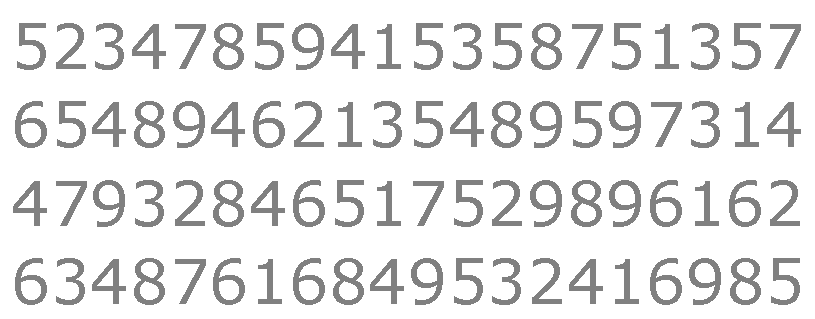
\includegraphics[width=0.8\textwidth]{obrazky-figures/fives.pdf}
\end{center}
\caption{Příklad efektu intenzity barvy na vnímání.}
\end{figure}

Z tohoto porovnání je na první pohled možné poznat, že na levém obrázku, kde nejsou číslice zvýrazněny je jejich nalezení daleko obtížnější, oproti tomu v pravém obrázku jsou číslice díky jejich zvýraznění možné hned odlišit. Důvod je jednoduchý, použité barvy jsou vysoce kontrastní. Kontrast, narozdíl od tvaru číslic je jeden z parametrů, který je vnímaný ve fázi předběžného zpracování. Tyto koncepty popisuje Colin Ware \cite{ware2012information} ve své knize.

\subsection{Gestalt principy}
Gestalt principy se zaměřují na to, jak lidský mozek vnímá vzory nebo konfigurace elementů. Původní německé slovo Gestalt je do češtiny překládáno jako podoba, tvar nebo struktura, odtud pochází alternativní název tvarová psychologie, který se často používá více v psychologii než v oboru informačních technologií. Tyto principy jsou pro vytváření jakýchkoli vizuálních prvků velmi důležité a proto se často používají jak pro dashboardy tak i jiné vizualizace, jako například animované vizualizace síťových dat \cite{1028859}.

Dobrým příkladem, který ukazuje proč jsou tyto principy důležité je takzvaný princip blízkosti, který nám říká, že objekty, které jsou blízko sebe máme tendenci vnímat jako jednu skupinu. Tohoto principu můžeme využít pro vytváření skupin, které budou velmi jednoduché na vnímání i bez použití dalších vizuálních prvků.

\section{Typy vizualizací}
Pro velké množství typů dat, které je nutné zobrazovat již existují efektivní nástroje, nebo způsoby, které mohou tvorbu dashboardu velmi usnadnit. Tyto způsoby je možné rozdělit do dvou kategorií na základě toho, pro jaký typ dat jsou více přizpůsobená a to na vizualizace, které zobrazují grafová data a vizualizace, která využívající mapu.

\subsection{Grafové}
V typických dashboardech je nejčastěji nutné zobrazovat kvantitativní data jako například různé teploty, průměrnou cenu zakoupených produktů v dané kategorii a další. Všechny prvky v této kategorii zobrazují 2D data, což reprezentuje problém. Data, která chceme zobrazovat mohou mít více dimenzí. V některých případech může zobrazení mnoha dimenzí ve vizualizaci způsobit nepřehledost dané vizualizace. Do této kategorie patří tradiční grafy sloupcové, spojnicové, odrážkové a takzvané sparklines.

\subsection*{Sloupcové grafy}
Tento typ grafu je vhodný zejména v tom případě, kdy je nutné zobrazit hodnoty měření, které spadají do nějaké kategorie. Hodnoty v tomto grafu jsou reprezentovány sloupci umístěnými v systému souřadnic, kde jedna osa reprezentuje danou kategorii, kde se může jednat například o nominální nebo ordinální hodnotu a druhá vlastní hodnotu této kategorie.
\begin{figure}[H]
\label{question4}
\begin{center}
    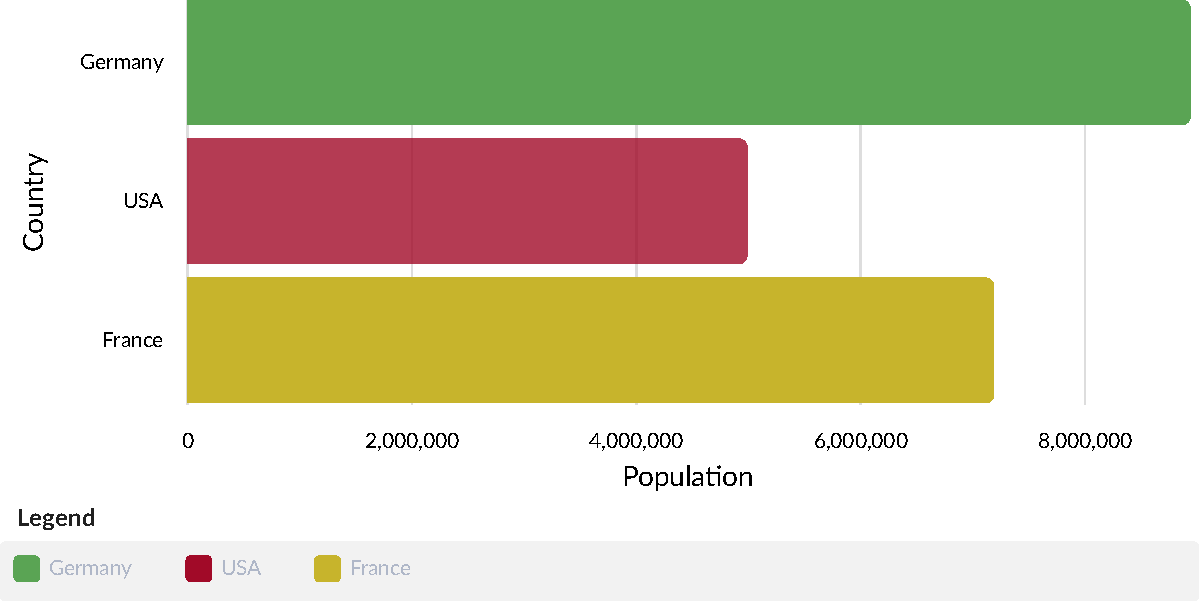
\includegraphics[width=0.8\textwidth]{obrazky-figures/bar.pdf}
\end{center}
\caption{Příklad sloupcového grafu, převzato z \protect\footnotemark}
\end{figure}
Podle umístění osy s kategorií se poté jedná o horizontální nebo vertikální sloupcový graf. Díky tomu zdůrazňování jednotlivých hodnot umožňuje tento graf zobrazené hodnoty a je proto častým kandidátem pro zobrazování dat ve strategických dashboardech.
\footnotetext{Ukázky grafů ngx-charts: \url{swimlane.github.io/ngx-charts/}}
\subsection*{Spojnicové  grafy}
Tento typ grafu je velmi praktický v případech, kdy je nutné podrobně zobrazit veličinu, která se například postupně vyvíjí v čase nebo je takto závislá na jiné veličině. Stejně jako předchozí typ využívají spojnicové grafy souřadnicový systém, na který vynáší spojnice dat. 
\begin{figure}[H]
\label{question4}
\begin{center}
    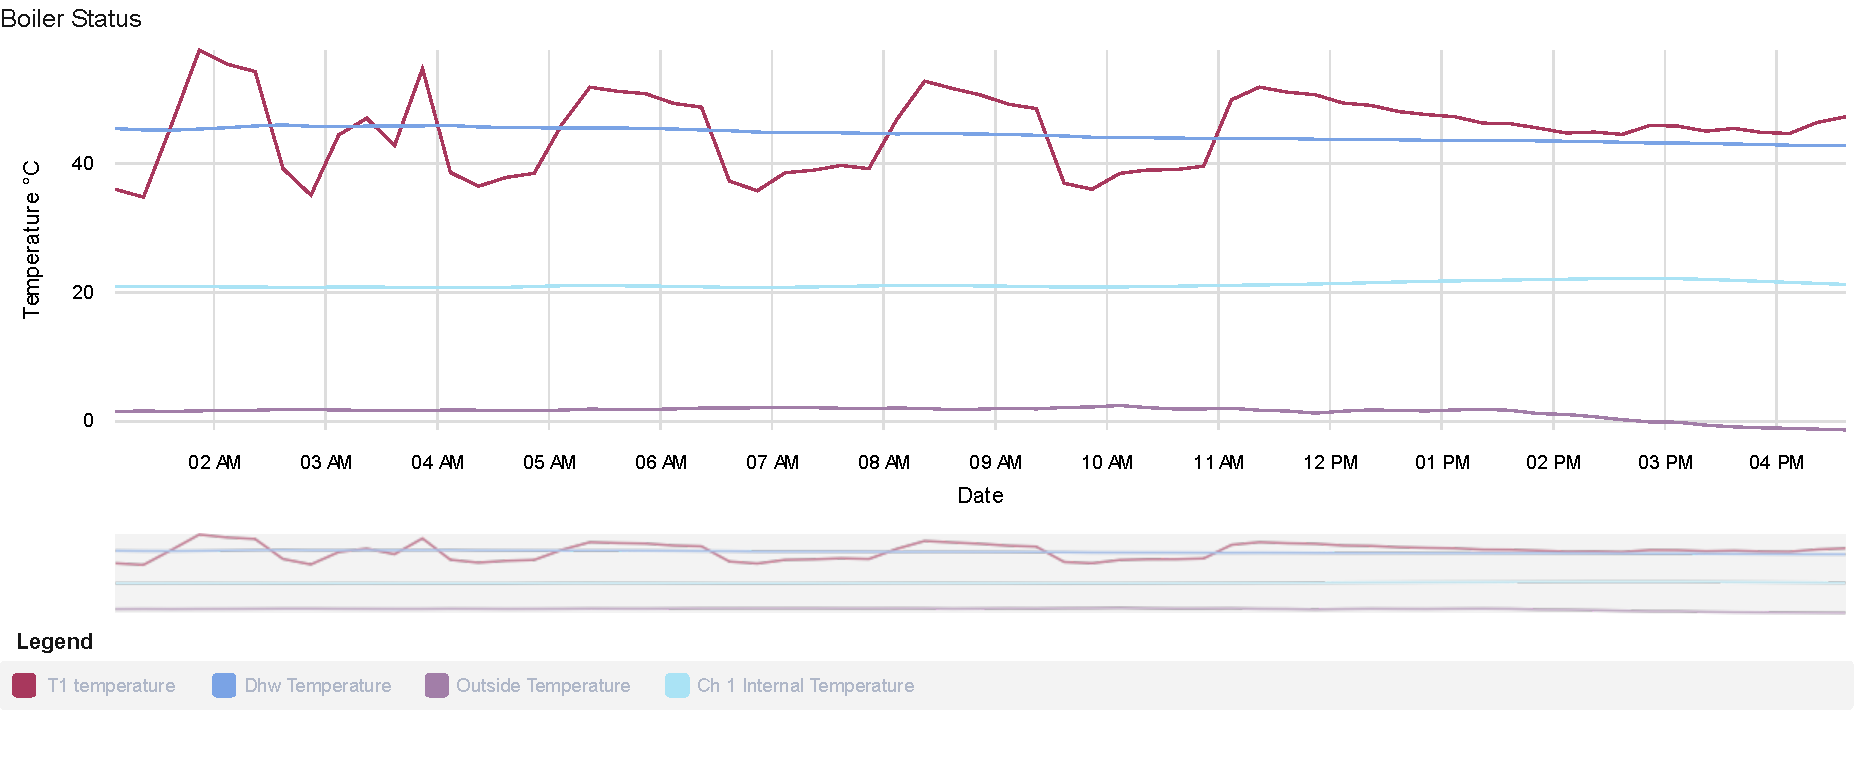
\includegraphics[width=0.8\textwidth]{obrazky-figures/line.pdf}
\end{center}
\caption{Příklad spojnicového grafu}
\end{figure}
Díky tomuto přístupu je možné na spojnicových datech dobře pozorovat trend zobrazované hodnoty. Na první pohled tedy můžeme zjistit, zdali daná hodnota roste, nebo naopak klesá nebo jak stabilní je. Tyto vlastnosti jsou žádoucí v dashboardech provozního typu.

\subsection*{Sparklines}
Sparkline je typ grafu, který je velmi podobný spojicovému grafu a je popisován jako \uv{jednoduchá, datově intenzivní grafiku o velikosti slova}. Na rozdíl od spojnicového grafu sparkline nepoužívá ani jednu osu. 
\begin{figure}[H]
\label{question4}
\begin{center}
    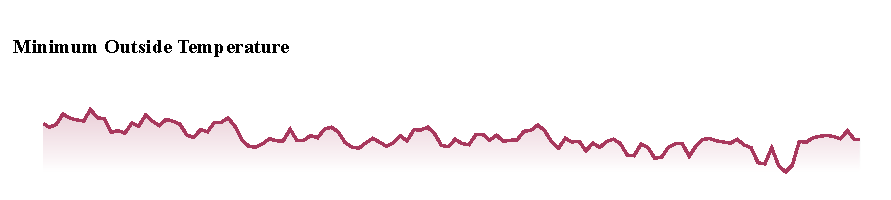
\includegraphics[width=0.8\textwidth]{obrazky-figures/sparkline.pdf}
\end{center}
\caption{Příklad sparkline}
\end{figure}
Tato vlastnost se může na první pohled zdát jako nevýhoda, ale díky tomu, že se grafy typu sparkline používají k zobrazení historických trendů, které jsou jasné z prvního pohledu jsou hlavně díky jejich malé velikosti při tvorbě dashboardů velmi praktické.

\subsection*{Odrážkové grafy}
Odrážkový graf, častěji nazývaný původním anglickým názvem \textit{bullet graph}, je speciální typ grafu, který představil Stephen Few \cite{few2004dashboard} za účelem odstranit nevýhody budíkového grafu. Tento a ostatní jemu podobné grafy zobrazují hodnotu pouze jedné veličiny často s porovnáním cílovou nebo předpovídanou hodnotou a nebo kvantitativní škálou. Podle autora budíkové a podobné grafy nevytváří nejjasnější a nejsmysluplnější reprezentaci dat, která by zabírala co nejmenší množství místa. Jako řešení navrhuje novou vizualizaci, která stejně jako sloupcové grafy využívá sloupců. Jeden z těchto sloupců vždy reprezentuje samotnou hodnotu a zbylé sloupce v pozadí reprezentují kvantitativní rozsahy dané hodnoty.

\begin{figure}[H]
\label{question4}
\begin{center}
    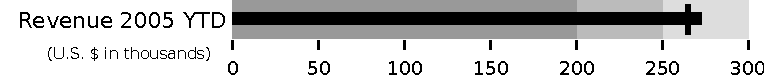
\includegraphics[width=0.8\textwidth]{obrazky-figures/Bullet_Graph_Example.pdf}
\end{center}
\caption{Příklad odrážkového grafu, převzato z \cite{few2004dashboard}}
\end{figure}

\subsection{Mapové}
Často je v dashboardech nutné zobrazit i data, která vyžadují drasticky jinou vizualizaci. Jedním z častých případů je danou vizualizací nějaký typ mapy. Může se jednat například o geografickou mapu zobrazující cestu zvoleného vozidla za zvolené období nebo o abstraktní mapu zařízení připojených k lokální síti. Tyto zobrazení jsou často velmi specifické k jejich použití a není jednoduché navrhnout konkrétní komponenty, které by bylo možné znovu použít jako v předchozích případech. 

\section{Klíčové ukazatele výkonnosti}
K vyhodnocení stavu systému nestačí pouze samotná data, ale je potřeba vytvořit speciální odvozené hodnoty. Tyto hodnoty se nazývají klíčové ukazatele výkonnosti (KPI), a slouží k vyhodnocení úspěšnosti organizace nebo akce. K tomu, aby byly tyto metriky přínosné pro danou společnost musí odpovídat strategii, kterou firma využívá. 

V dnešní době není vždy nutné vytvářet nová KPI, ale spíše vybírat z předem připravených kolekcí, jakou je například kniha \cite{marr2012key} Bernarda Marra, ve které je prezentováno 75 KPI pro použití manažery. V některých případech ale není výběr tak jednoduchý. Jedním z těchto případů jsou například komunitní KPI pro chytrá města, kdy je nutné vyhovět požadavkům nejen samotné společnosti ale také jednotlivých uživatelů systémů poskytovaných městem s ohledem na jejich soukromí. Touto problematikou se zabývali Drew Hemment, Mel Woods, Vimla Appadoo a Lily Bui, kteří ve své zprávě \cite{hemment2016community} presentovali způsob vytvoření komunitních KPI ve městě Manchester v rámci projektu CityVerve. 
Vytváření KPI je v této zprávě rozděleno do následujících 4 fází:
\begin{itemize}
\item Návrh cílů -- je zaměřen na objevování a definování cílů a k nim potřebných KPI. Výsledkem jsou vysokoúrovňové KPI ze kterých budou odvozeny KPI pro individuální projekty.
\item Iterace procesu -- je zaměřena na vylepšení a upřesnění jednotlivých KPI založené na bližším popisu.
\item Vytváření aktiv -- je zaměřeno na způsoby integrace nových KPI do již existujícího projektu.
\item Vyhodnocení -- obsahuje hodnocení finálního řešení a pochopení nově získaných zjištění.
\end{itemize}
Do celého procesu jsou zahrnuti nejen zástupci společnosti, která dodává programové řešení a členové městského zastupitelstva, ale také obyvatelé samotného města.

K zobrazení hodnot KPI se často využívají vizualizace, které byly představeny v předchozí kapitole, ale jen některé z nich jsou efektivní pro dané použití. Efektivitu dané vizualizace je proto nutné vždy zvážit a zhodnotit. Například Yorick Heidema se v jeho diplomové práci \cite{heidema2018visualizing} zabývá hodnocením vizualizací KPI pro produkční plánování ve výrobě. V některých případech je dokonce nutné poskytovat data jiným způsobem, než za pomocí dashboardů a to například zasláním zprávy, která obsahuje potřebné vizualizace uživateli \cite{hemment2016community}.
\section{Detekce anomálií}
Jak už bylo několikrát zmíněno data ze senzorů mohou být určitým způsobem zašuměná nebo jiným způsobem nekvalitní. Nekvalitní data mohou obsahovat hodnoty, které jsou mimo měřitelný rozsah zařízení k čemuž často dochází při spuštění zařízení, kdy byla odečtena hodnota senzoru dříve, než došlo k prvnímu měření senzoru. 

Data také mohou obsahovat chybějící nebo odlehlé hodnoty. Odlehlé hodnoty mohou být důležitá i pro detekci rychlých a neočekávaných změn v systému, které nemusí naznačovat pouze chybu systému, ale také například jeho netradiční chování.

Kontrolu dat na již zmíněné nedostatky není možné provádět ručně a to z velmi jednoduchého důvodu. Data z IoT zařízení jsou příliš rozsáhlá a přibývají velmi rychle. Proto je nutné se s některými nedostatky automaticky vypořádat pokud možno již při samotném vkládání dat tak, aby nebyla ovlivněna odvozená data. Občasné výpadky je možné doplnit aproximací založenou na předchozí a následující hodnotě a hodnoty mimo měřený rozsah mohou být ignorovány a nebo uloženy do jiné databáze, která je k tomuto účelu vyhrazena.

Mezi anomálie, které se tradičně detekují v časových sériích \cite{laptev2015generic, ren2019time} patří odlehlé hodnoty, takzvané body změny a anomální časové série.
\subsection*{Odlehlé hodnoty}
Detekování odlehlých hodnot bývá často považováno jako nejdůležitější typ detekce anomálií. Detekce těchto hodnot se často provádí dvěma způsoby a to buď modelováním tradičního chování této časové série nebo pomocí metod založených na dekompozici.

První způsob k detekci využívá dvou částí a to algoritmu, který slouží k předpovědi a algoritmu, která vypočítá relativní chybu mezi předpovídanou a naměřenou hodnotou. Pokud je poté tato relativní chyba mezi hodnotami větší než uživatelem zadaný práh, je naměřená hodnota označena jako odlehlá. 

Tato metoda často produkuje dobré výsledky na sériích, které nevykazují náhlé změny a je možné je namodelovat způsobem, který dobře odráží realitu. Pokud ale časová série obsahuje časté výkyvy bude tato metoda detekovat velké množství falešně pozitivních hodnot.

Dekompoziční metoda poté rozděluje časovou sérii na trend, sezónní data a šum. Právě v šumu jsou poté detekovány odlehlé hodnoty na základě prahu zadaného uživatelem.
\subsection*{Body změny}
Body změny odpovídají momentům, kdy se mění chování dané časové série z očekávaného na neočekávané. Na rozdíl od odlehlých hodnot tento bod označuje trvalejší změnu.

Jeden ze způsobů, jak tyto změny detekovat, představují metriky rozdílnosti založené na posuvném okénku, které srovnávají rozdíly získaných dat ve dvou po sobě následujících okénkách. Tyto techniky jsou často nazývány jako takzvané absolutní techniky protože nevyužívají žádných předpokladů k vyhodnocení.

Druhým způsobem jsou metody relativní nebo metody založené na modelech. Tyto metody se snaží předpovědět očekávané chování.  Datové vzorky, které neodpovídají předpovídaným hodnotám jsou poté nazývány jako zbytkové hodnoty a to, jestli obsahují body změny je vyhodnoceno pomocí absolutních technik.
\subsection*{Anomální časové série}
Poslední anomálii představují anomální časové série. Střední odchylka těchto sérií je často výrazně rozdílná od ostatních podobných časových sérií v systému. 

Tuto detekci je možné provést vytvořením shluků z podobných časových sérií, které je možné vytvořit například autokorelací nebo spektrální entropií. V takto vytvořených shlucích je poté možné detekovat anomální časové série pomocí výpočtu střední odchylky mezi těžišti jednotlivých časových sérií.

\chapter{Uživatelská rozhraní a vizualizace dat}
\label{chapter_visualisation}
Po uložení dat a vytvoření návrhu dashboardů je nutné vybrat technologie k jejich implementaci. V dnešní době je velmi praktické vytvářet informační systém s dashboardy jako webovou aplikaci, což dovoluje uživatelům zobrazit potřebná data na prakticky jakémkoliv zařízení připojeném k internetu. 

Populární je provádět samotné sestavování výsledné stránky na klientovi, což je sice limitující z pohledu použití technologií a nutnosti implementovat kontrolu uživatelských vstupů jak na serveru tak na klientovi. Na druhou stranu tento přístup přináší možnost přesunout podstatnou část výpočtu právě na klienta.

K vytvoření zmíněných vizualizací je možné použít nástroje, které jsou vestavěné do všech moderních webových prohlížečů, které podporují standard HTML5 a elementy \textit{canvas} a \textit{svg} v kombinaci s programovacím jazykem JavaScript, nebo jeho rozšířením TypeScript. Oba dva typy elementů je možné při vytváření vizualizací využít, ale vektorová grafika v podobě svg nám oproti rastrovému elementu canvas přináší možnost vytvářet grafiku, kterou bude možné lépe přizpůsobovat konkrétním zařízením uživatele. U obou přístupů je ale vytváření tradičních vizualizací jejich přímým použití velmi pracné a to nejen v případě vykreslování, ale hlavně předzpracování dat. Oba tyto problémy řeší populární knihovna D3.js.

\section{D3.js}
Tato knihovna\footnote{Domovská stránka projektu \url{https://d3js.org/}} poskytuje nízkou míru abstrakce, ale velmi dobrý výkon. Své reprezentace vytváří pomocí standardních HTML prvků díky čemuž je možné zajistit vysokou kompatibilitu napříč různými webovými prohlížeči. I přes to, že je knihovna D3.js typicky používána v programovacím jazyce JavaScript existují pro ni i takzvané typové definice, které dovolují vytvářet nové vizualizace pomocí programovacího jazyka TypeScript, což omezí chyby vzniklé špatným použitím knihovny. I přesto, že D3.js obsahuje vestavěné způsoby vizualizace se spíše jedná o matematickou knihovnu, která poskytuje velké množství funkcí pro předzpracování dat.

Knihovna D3.js velmi oblíbená při vytváření specializovaných řešení, pro které ještě nebyly navrženy abstraktnější knihovny, nebo právě při tvorbě nových knihoven. Z vytvořených vizualizací je velmi praktické vytvořit komponenty, které bude možné znovu používat jak v rámci aplikace tak napříč dalšími aplikacemi.

\section{Technologie pro vizualizaci dat}
Vytvořené komponenty nemusí obsahovat pouze vizualizace dat, ale také zbylé prvky uživatelského rozhraní. Po tomto rozdělení bude možné výsledné uživatelské prostředí tvořit kompozicí vzniklých komponentů, které bude jednodušší na údržbu díky jejich malé velikosti. Tyto znovu použitelné komponenty je zajisté možné vytvářet ručně, ale častějším případem je využití některé z dostupných a velmi populárních knihoven, které tento proces velmi zjednodušují.

Mnoho knihoven přináší kromě možnosti vytvoření komponentů i další funkce, které mohou být při vytváření uživatelských rozhraní velmi užitečné. Dobrým příkladem přidané funkce jsou šablonovací jazyky, nebo možnosti jednoduše obsloužit interakce uživatele s jednotlivými komponenty. Mezi často používané knihovny patří React a Angular.

\subsection*{React}
React\footnote{Domovská stránka projektu \url{https://reactjs.org/}} je velmi populární a minimalistický aplikační rámec vyvíjený společností Facebook. Aplikace v něm vytvořené se skládají pouze z komponentů, které mají definovaný vzhled ve speciálním jazyce JSX\footnote{Více o jazyce JSX \url{https://reactjs.org/docs/introducing-jsx.html}}. Díky tomuto speciálnímu jazyku je možné kombinovat strukturální zápis HTML s kódem v jazyce JavaScript, který dovoluje obsluhovat akce uživatele. 

Jak již bylo zmíněno tento aplikační rámec je velmi minimalistický a proto je často potřeba ho rozšířit o další funkčnost. Díky jeho popularitě tohle nečiní výrazný problém a existuje velká řada komunitních rozšíření, z nichž jsou některá dokonce i doporučená.

\subsection*{Angular}

Angular\footnote{Domovská stránka projektu: \url{https://angular.io/}} je komplikovanější aplikační rámec, který vyžaduje přesnou strukturu a využití jazyka TypeScript, ale poskytuje robustní způsob k vytvoření webových aplikací. Stejně jako React i Angular rozděluje části vzhledu na komponenty, ale narozdíl od něj mají samotné komponenty pevně předepsanou strukturu, která od sebe odděluje strukturu, vzhled a samotnou funkčnost. 

Kromě samotných komponentů poskytuje Angular další nástroje, které zjednodušují aspekty, které je často nutné řešit při vytváření frontendových webových aplikací zavedením vyšší míry abstrakce, kterou je velmi jednoduché použít. Příkladem této abstrakce může být zjednodušení komunikace mezi serverem a klientem přes takzvané \textit{Observers}, které dovolují jednoduše získávat data ze serveru a současně na jejich základě jednoduše aktualizovat jednotlivé komponenty.

\section{Vizualizace tradičních dat}
Podobný přístup již před námi zvolilo více vývojářů, takže už existují knihovny, které obsahují časté typy vizualizací. Jednotlivé vizualizace jsou poté reprezentovány jako samostatné komponenty, které jsou přizpůsobeny pro některou z vizualizačních knihoven. 

Využitím těchto knihoven můžeme zrychlit vývoj samotné aplikace, ale musíme zvolit knihovnu, která podporuje nejvíce z požadovaných vizualizací, nebo více knihoven s tím, že jsme připraveni v případě potřeby upravit vzhled jednotlivých prvků vizualizací. Tuto situaci velmi zjednodušují knihovny, které dovolují jednoduše změnit svůj vzhled.

\subsection*{Ngx-charts}
Ngx-charts\footnote{Domácí stránka projektu: \url{https://github.com/swimlane/ngx-charts}} je deklarativní knihovna, která vytváření svých vizualizací využívá knihovny D3.js a Angular. Tuto knihovnu vyvíjí společností Swimlane\footnote{Oficiální stránky společnosti: \url{https://swimlane.com/}} jako software s otevřeným zdrojovým kódem. Narozdíl od mnohých ostatních knihoven ale tato knihovna nemění pouze vzhled výsledných komponent nebo grafů, ale využívá vlastního jádra, matematických funkcí a generátorů obsažených v D3.js a datových vazeb aplikačního rámce Angular k vytvoření vlastních komponentů a vizualizací. Všechny komponenty jsou také zpřístupněny přímo v modulu, díky čemuž je možné je velmi jednoduše využít při vytváření vlastních grafů a vizualizací.

\subsection*{Carbon Charts}
Carbon Charts je aplikační rámec vytvoření firmou IBM jako část jejich návrhového systému Carbon\footnote{Oficiální stránky návrhového systému \url{https://www.carbondesignsystem.com/}}. Tento návrhový systém se snaží poskytnout kolekci předpřipravených, znovu použitelných komponentů a vzorů pro zrychlení vývoje. 

Carbon Charts narozdíl od aplikačního rámce Ngx-charts vytváří své vizualizace využitím D3.js a vlastních stylů, ale přidává i další a pokročilejší vizualizace, které Ngx-charts neposkytuje, jako je například stromové vizualizace nebo základní geografické vizualizace. Dalším důležitým rozdílem je i platforma. Jelikož se jedná o součást návrhového systému existují verze pro mnoho aplikačních rozhraní pro tvorbu uživatelských rozhraní včetně již zmíněného Reactu a Angularu, ale i pro použití bez nich.

\section{Grafana}

Grafana je multiplatformní webová aplikace s otevřeným zdrojovým kódem, která poskytuje možnost rychle vytvářet vlastní dashboardy a jiné pohledy z velké množiny databázových systémů nebo jiných zdrojů dat. Narozdíl od předchozích technologií je u této aplikace daleko jednodušší začít rychle provozovat a to díky možnosti spustit aplikaci přímo v cloudu výrobce nebo spuštění již hotové aplikace lokálně. Grafana poté dovoluje vytvářet dashboardy přímo v aplikaci a to jednoduchým výběrem.

Tímto faktem vybočuje od předchozího rozdělení. Zatímco u předchozích řešení bylo vždy nutné vytvářet vlastní webovou aplikaci Grafana poskytuje možnost rychlého velmi nasazení, což může být velmi praktické například v případě, kdy je nutné začít data vizualizovat co nejrychleji.

Kromě již hotové aplikace je možné využít komponentů vytvořených pomocí aplikačního rámce React při vytváření vlastní aplikace. Kromě vestavěných vizualizací existuje i velká řada komunitních rozšíření. 

\section{Vizualizace geografických dat}
Oproti vizualizaci tradičních dat se vizualizace geografických dat významně liší. Zatímco v případě tradičních dat je předzpracování relativně jednoduché u geografických dat musíme počítat s kulovitým tvarem země. Z tohoto důvodu se používají projekce. Tyto operace transformují zploštělé koule do dvoudimenzionálního prostoru. I o předzpracování geografických dat se stará část knihovny D3.js s názvem d3-geo.

Stejně jako v předchozím případě i pro geografická data existuje mnoho aplikačních rámců, které poskytují velké množství již předpřipravených řešení, které je možné použít. Stejně jako v předchozím případě existují aplikační rámce s otevřeným zdrojovým kódem, ale velmi populární bývají i proprietární a placená řešení například v podobě Google Maps. Tato sekce je zaměřená pouze na aplikační rámce s otevřeným zdrojovým kódem.

\subsection*{Leaflet}
Leaflet je knihovna založená na jazyce JavaScript a poskytuje možnost vytvářet jednoduchá a velmi výkonná řešení, která budou efektivní i na zařízeních s dotykovou obrazovkou jako jsou například chytré mobilní telefony. K vytváření vizualizací tato knihovna využívá standardních HTML elementů, díky čemuž je velmi jednoduché změnit vzhled nebo další vlastnosti finálního zobrazení.

K vytváření svých zobrazení Leaflet využívá nízkoúrovňové funkce obsažené v d3-geo, ale i přes značné zjednodušení vyžaduje dobrou znalost jazyka JavaScript. Základní balíček obsahuje pouze nástroje pro tvorbu a práci se samotnou mapou, pro jakékoli složitější použití je možné použít velké množství již existujících rozšíření, která jsou vyvíjena velmi aktivní komunitou.
\subsection*{Geovisto}
Geovisto je knihovna vyvíjená naší fakultou\footnote{Webová stránka produktu Geovisto \url{https://www.fit.vut.cz/research/product/669/.cs}} založená na rámcích Leaflet a D3.js a rozšiřuje možnosti, které Leaflet podporuje. K vytvoření mapy je využit aplikační rámec Leaflet a k vytváření vizualizací nad tímto podkladem slouží D3.js. Jednotlivé vizualizace jsou uspořádány do vrstev, díky čemu je možné zpracovávat a vizualizovat vícevrstvá geografická data.

Hlavní výhodou je způsob ovládání knihovny. Zatímco Leaflet vyžaduje znalost jazyka JavaScript Geovisto je založené na deklarativním způsobu čímž usnadňuje vytváření vizualizací. Knihovna jako taková je velmi modulární, díky čemuž je možné stahovat používat pouze ty části, které jsou potřeba nebo velmi jednoduše vytvářet další potřebná rozšíření.

\chapter{Analýza}
\label{chapter_analysis}
Po zvolení technologií pro ukládání a zobrazování dat je také nutné zvolit data, která budou v jednotlivých pohledech zobrazována a vybrat způsoby, jak se vypořádat s nekvalitními daty, nebo jak detekovat odlehlé hodnoty v nich. Za tímto účelem je nutné pochopit nejen povahu daných dat, ale i to, jakým způsobem budou využívány koncovými uživateli a jak je obtížné tyto data získat.

Cílová skupina uživatel velmi ovlivňuje data, která bude potřebné zobrazit. Z tohoto důvodu je nutné pochopit cílovou skupinu uživatel. V  tomto případě již v současné době existuje řešení, které je nutné analyzovat, najít a opravit jeho případné nedostatky. 

\section{Logimic}
Logimic\footnote{Oficiální stránky společnosti: \url{https://www.logimic.com/}} je česká firma, která se vytváří IoT systémy pro průmyslové účely a to nejčastěji pro sledování a nebo řízení. Firma se hlavně zaměřuje na bezdrátový přenos dat a ovládacích příkazů k zařízením a svým zákazníkům poskytuje nejen návrh systémů, ale i samotné hardwarové i softwarové řešení, cloudovou infrastrukturu a odborné konzultace. K provozu cloudových řešení Logimic využívá již zmíněnou službu AWS od firmy Amazon. Díky tomuto přístupu může firma jednoduše poskytovat služby s vysokou dostupností, z velké části vyřešeným zabezpečením a nízkou odezvou prakticky po celém světě. 

Data z chytrých zařízení jsou přenášena v podobě MQTT zpráv do takzvané AWS Lambda, která dovoluje zápis do databází bez využití stále běžícího serveru. Odpovídající kód se vykonává pouze v případě, že je to zapotřebí, jinak zůstane serializován na disku. Příchozí data jsou následně předzpracována a zapsána do dvou databázových systémů a to PostgreSQL a DynamoDB.

Získaná data jsou uživatelům dodaných systémů zobrazována frontedovou aplikací založenou na již zmíněném aplikačním rámci Angular. Získávání dat z databázových systémů probíhá podobným způsobem jako jejich zápis. Při výběru je tedy kontaktována odpovídající lambda, která autentifikuje a autorizuje uživatele a pokud je k dané operaci oprávněn vyhodnotí daný dotaz. Časové série jsou získávány z databázového systému DynamoDB, což přináší již popsané nevýhody. 

\begin{figure}[H]
\label{question4}
\begin{center}
    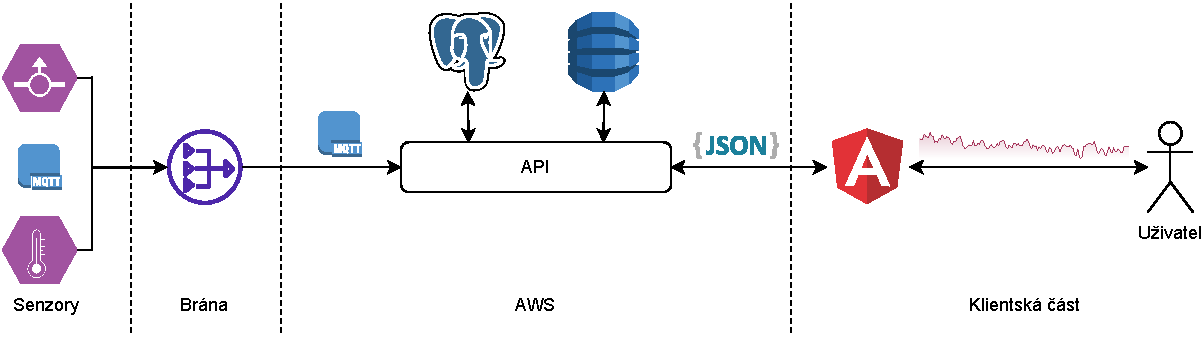
\includegraphics[width=0.9\textwidth]{obrazky-figures/DIP-architecture.pdf}
\end{center}
\caption{Schéma popisované architektury}
\end{figure}

Tyto nevýhody jsou velmi omezující při tvorbě dashboardů, které využívají velkého množství dat, nebo vyžadují výpočet jiných hodnot a to například agregací. Dále také představují značné omezení v případě, že by se firma rozhodla některému ze svých zákazníků zřídit systém v interní infrastruktuře a prostoru zákazníka. Za tímto účelem je v současné době testován přechod na již zmíněný databázový systém InfluxDB, který je pro toto použití lépe přizpůsobený.

\section{Současný stav}
V současném stavu odpovídá velká část poskytovaných dashboardů analytickému typu. Uživateli jsou nejdřív zobrazeny agregované pohledy nejdůležitějších KPI daného typu senzoru. Pokud jsou hodnoty všech KPI v této skupině v nastaveném rozsahu jsou odpovídající vizualizace podbarveny zelenou barvou. Pokud je ale některá z hodnot mimo daný rozsah je vygenerováno upozornění a je změněna barva na úvodním dashboardu.

\begin{figure}[H]
\label{question4}
\begin{center}
    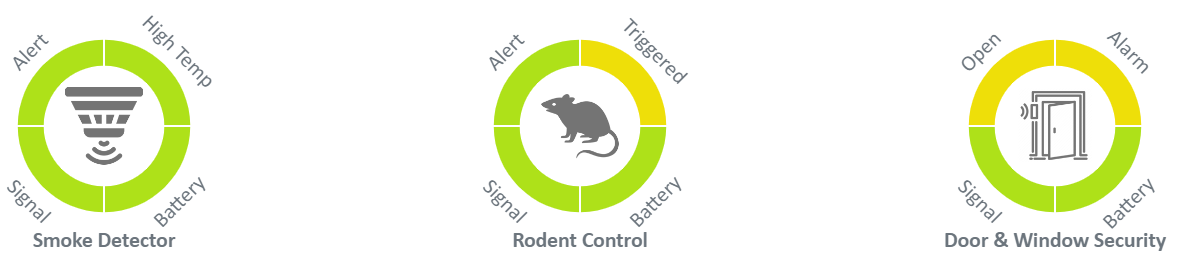
\includegraphics[width=0.25\textwidth]{obrazky-figures/l1.png}
\end{center}
\caption{Zobrazení skupiny KPI}
\end{figure}

Po kliknutí na vizualizaci je možné přejít k méně agregovanému pohledu, kde vidíme detail každé kategorie KPI. V tomto přehledu jsou zobrazeny všechny skupiny KPI podobných způsobem jako v předchozím pohledu. 

\begin{figure}[H]
\label{question4}
\begin{center}
    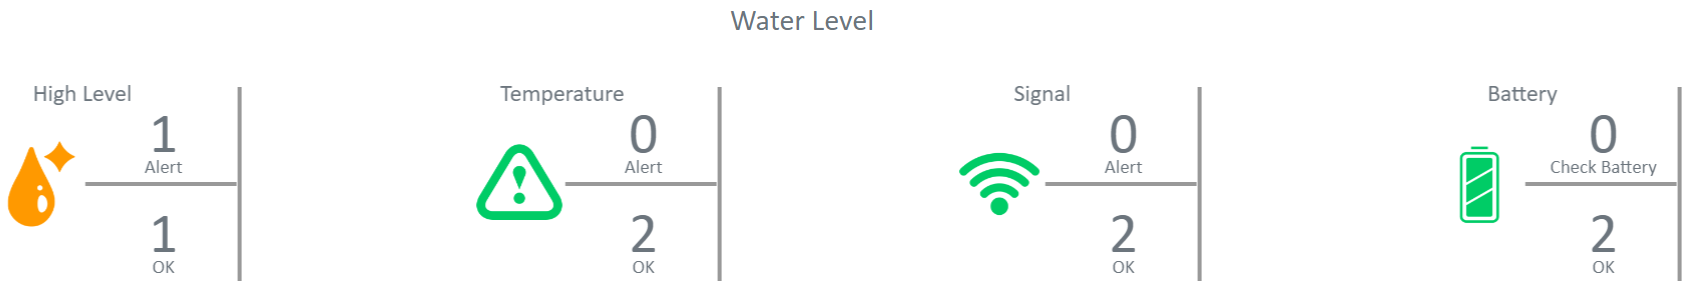
\includegraphics[width=0.9\textwidth]{obrazky-figures/l2.png}
\end{center}
\caption{Zobrazení agregovaných KPI ve skupině}
\end{figure}

V neposlední řadě je možné se zanořit na nejnižší úroveň a sledovat samotné hodnoty jednotlivých zařízení. V současné době je tato část dashboardu ve vývoji a jedná se pouze o její prvotní návrh. 

\begin{figure}[H]
\label{question4}
\begin{center}
    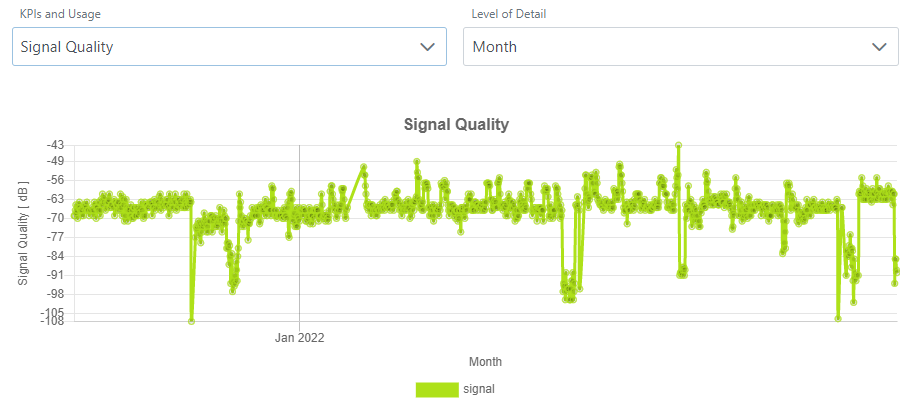
\includegraphics[width=0.9\textwidth]{obrazky-figures/l4_stats.png}
\end{center}
\caption{Detail konkrétních hodnot zvoleného zařízení}
\end{figure}

Toto zobrazení dovoluje vybrat jednu z měřených hodnot senzoru a zobrazit její průběh za zvolené časové období. Průběh je zobrazen ve formě interaktivního spojnicového grafu, kdy je po najetí na část grafu získat odpovídající hodnotu v daném čase. Dále také nejnižší úroveň obsahuje textové informace o samotném senzoru a přehled rychlý přehled aktuálních informací a vybraných agregovaných hodnot.

\begin{figure}[H]
\label{question4}
\begin{center}
    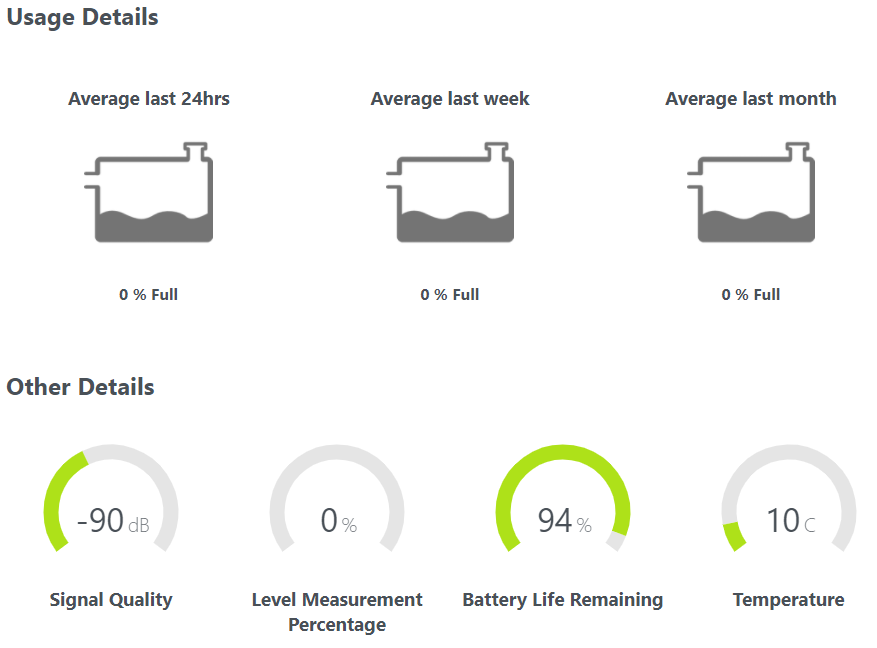
\includegraphics[width=0.9\textwidth]{obrazky-figures/l4_extras.png}
\end{center}
\caption{Přehled agregovaných hodnot zvoleného zařízení}
\end{figure}

Z velké části jsou zmíněné vizualizace efektivní pro zobrazení vyžadovaných dat. Výjimkou je zobrazení samotných hodnot zařízení, které může být v některých případech neefektivní. Například při zobrazení dlouhého časového úseku dojde k načtení velmi velkého počtu neagreagovaných vzorků. Počet vzorků způsobí zvýšení potřebného výkonu jak pro zařízení uživatele tak pro server poskytující data. Ideálním řešením by bylo zvolit úroveň agregace automaticky na základě délky zvoleného časového období, které by mohl uživatel ručně změnit.

Časové období, ve kterém se uživateli zobrazují data je možné zvolit pouze z předdefinovaných hodnot týden, měsíc a rok. Tento fakt přináší další limitaci. V některých případech může být pro uživatele potřebné zobrazit časové období, které neodpovídá žádné z těchto možností. 

Poslední pro uživatele zajímavou funkcí by mohla být možnost srovnat data dvou zařízení, nebo data stejného zařízení v odlišném období. Například tedy srovnání průběhu teploty stejného senzoru ve stejném měsíci jiného roku.

V současné době systém neprovádí žádnou ze zmíněných kontrol odlehlých hodnot. Tyto hodnoty, je ale stále možné detekovat, protože bude vyhodnocena v rámci KPI.

\chapter{Návrh}
\label{chapter_desing}
Po provedení analýzy aktuálního stavu je nutné nahvrhnout možná efektivní řešení. Tato řešení se budou týkat jak problému zobrazení dat ze senzorů tak jejich efektivního ukládání a zpracování. Po zvolení řešení obou problémů je nutné i zvolit způsob, který budou tyto aplikace propojeny. Operace by bylo možné provádět přímo ze zobrazení, ale tento přístup není praktický pro reálné použití.

Tato kapitola je rozdělena na tři části, kde každá představuje řešení jednoho z problémů. I přes to, že spolu tyto problémy souvisí existují různé způsoby řešení, které na sobě nejsou závislé.

\section{Ukládání a zpracování dat}
Při zpracování dat je nutné vzít v úvahu i jiná data než časové série senzorů. Tyto data mohou představovat například neměnné metadata o samotném senzoru, jako například název, identifikátor senzoru nebo jednotky, ve kterých daný senzor měří svá data, ale i ostatní informace, které jsou potřebné pro běh samotného informačního systému jako například informace o uživatelích. 

Jedním ze způsobů, jak se postavit k uložení obou typů dat by bylo vybrat jedinou databázi, která by sloužila k uložení obou typů dat. V případě použití relační databáze se musí počítat s problémy popsanými v kapitole \ref{chapter_db}. I na straně NoSQL databází není jednoduché vyřešit tento požadavek a to zejména kvůli malému výkonu relací. Ty je možné vyřešit denormalizací, to ale přináší své vlastní problémy, kterými je kromě velikosti i nutnost aktualizovat záznamy, které mohou být několikrát redundantně obsaženy i v několika tabulkách.

Jako lepší možnost připadá v úvahu použití dvou databázových systémů, kde jeden slouží pouze k uložení časových sérií a druhý, často relační databázový systém, slouží k uložení ostatních dat. Přístup k časovým sériím se může lišit. V některých systémech může být výhodné použít dokumentovou NoSQL databázi, ve které budou části sérií reprezentovány dokumentem v formátu, který bude přesně odpovídat konkrétnímu využití.

Tento přístup poskytuje velmi vysoký výkon za cenu prostoru a omezení ve volnosti výběrů. Druhým způsobem je využít takového NoSQL systému, který dokáže efektivně pracovat s časovými sériemi. Tento přístup je pro firmu logimic nejpřístupnější. Jak již bylo zmíněno firma využívá relační databázi pro ukládání dat. I přes to, toto řešení poskytuje možnost efektivně provádět agregace nad daty může být praktické ukládat hodnoty složitější operací. 

\begin{figure}[H]
\label{question4}
\begin{center}
    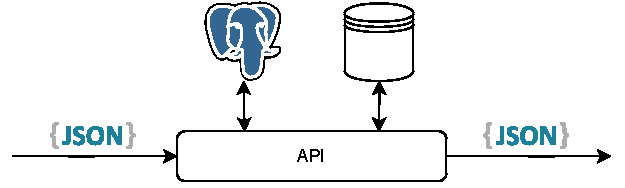
\includegraphics[width=0.9\textwidth]{obrazky-figures/databaseArchitecture.pdf}
\end{center}
\caption{Navrhovaná databázová architektura}
\end{figure}

Tyto hodnoty mohou být uloženy jak do zvoleného NoSQL systému tak do relační databáze. Pokud budou tato data ukládána dlouhodobě je efektivnější data ukládat zpět do NoSQL systému, kde mohou být v případě nutnosti znovu využita, nebo minimálně efektivně uložena. Naopak data, která jsou určena pouze k jednomu zobrazení, například aktuální hodnota senzoru, která bude pokaždé zobrazena ve vizualizaci, je efektivnější uložit do relační databáze.

V případě velkého zvýšení počtu požadavků by bylo možné relační databázi škálovat pomocí principu CQRS. Za tímto účelem by bylo nutné přidat do systému další NoSQL databázi, nebo jiné úložiště určené k rychlému čtení a zápisu. Vkládání, úpravu nebo mazání dat, tzv. příkazy, obslouží model zápisu, který zajistí propagaci změn do obou databázových systémů.

\begin{figure}[H]
\label{question4}
\begin{center}
    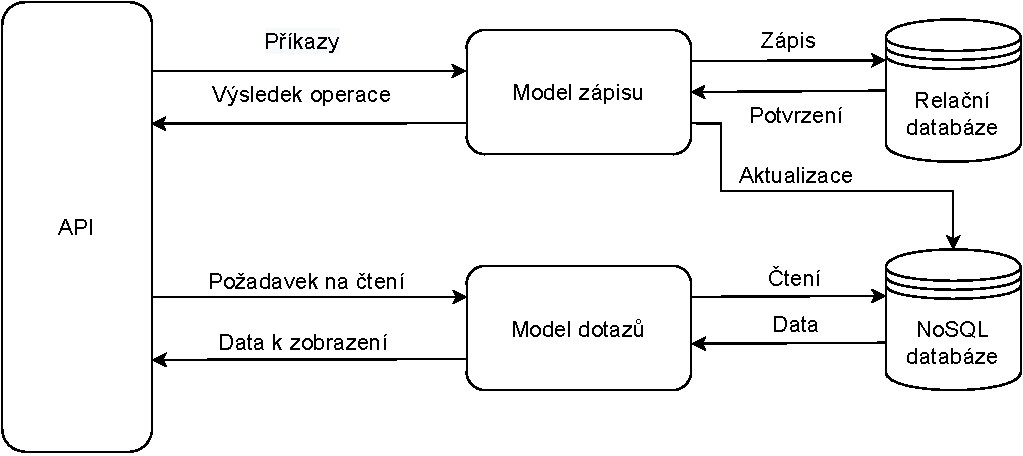
\includegraphics[width=0.9\textwidth]{obrazky-figures/csqr.pdf}
\end{center}
\caption{Architektura při použití principu CQRS}
\end{figure}

Databázový systém určený k ukládání časových sérií je možné škálovat přidáním odpovídajících uzlů s replikací, nebo exkluzivním rozdělení dat mezi více instancí zvolené databáze pro uložení časových sérii. V případech extrémně častého čtení by také bylo možné využít princip CQRS.

Se stále zvyšujícím se počtem vzorků v databázi bude narůstat její velikost. Tento problém má jednoduché řešení. Často nás zajímají přesné záznamy pouze u aktuálních dat. Čím jsou data poté starší tím se můžeme spolehnout na více nepřesné vzorky a staré vzorky můžeme odmazat z databáze úplně. Tyto operace jsou často podporovány v NoSQL databázových systémech a u senzorů, kde odmazání dat nepřináší žádné nevýhody doporučuji těchto možností využít.

\section{Návrh zobrazení}

Vytvořené zobrazení skupin KPI a stupňů zanoření je efektivní pro zobrazení vysokoúrovňových dat v aktuálním stavu. Horší situace je v případě zobrazení statistik konkrétního zařízení. Tyto statistiky jsou velmi jednoduché a dovolují zobrazit pouze jednu hodnotu zařízení. Toto je velmi limitující například v případě, kdy uživatele zajímá vztah více hodnot a to například v závislosti jedné hodnoty na druhé, jako tomu může být v případě vnitřní a venkovní teploty.

Žádným způsobem také není možné srovnat hodnoty dvou zařízení stejného typu. Toto zobrazení je méně důležité než jmenované předchozí a hodnoty zařízení ve stejné skupině je do jisté míry možné pomocí nastavení stejných limitních hodnot KPI. Toto srovnání by bylo více praktické vyřešit například zobrazením hodnot dvou senzorů stejného typu v jednom grafu. U kvantitativních nominálních hodnot je implementace tohoto srovnání jednoduchá a je možné ji provést zobrazením dvou nebo více spojnic spojnicového grafu. Větším problémem je způsob srovnání hodnot v ostatních případech. Například u senzoru stavu otevření dveří může být zajímavé srovnat využití dveří. Toto srovnání by bylo možné provést na základě srovnání počtu změn stavu senzoru.

Samotná frekvence změny stavu ale není dostatečným indikátorem využití. u předchozího příkladu mohou dveře zůstat například otevřené při velkém počtu lidí, kteří procházejí. Situaci neřeší dokonce ani kombinace obou těchto faktorů. Podobná situace je u více složitých požadavků. Vytvořené řešení by vždy bylo velmi závislé na problémů, který má řešit, takže by nebylo možné rychle přidávat a zprovozňovat a udržovat nová zařízení. 

Kvůli těmto limitacím je jediným řešením se snažit co nejvíce použít generické prvky zobrazení, kde by si uživatel mohl zvolit operaci, kterou chce nad zvolenou datovou sadou provést. Konkrétním příkladem může být spojnicový graf, který umožní uživateli zvolit konkrétní pole senzoru, časově období a agregační operaci, která má být použita. 

Tato vizualizace může tento problém vyřešit z numerických dat. U jiných typů dat může být užitečnější omezit uživateli výběr typu agregace a zobrazit v grafu pouze momenty, kdy dojde ke změně stavu. Tyto změny mohou být zobrazeny použitím spojnicového grafu, nebo jiným, speciálním typem, který by se podobal sloupcovému grafu s jedním sloupcem. Tento sloupec by byl rozdělen na segmenty podle časů jednotlivých změn.

V případě některých zařízení by také mohlo být prospěšné zobrazit jeho celkovou dostupnost. Výpočet dostupnosti může být založen na počtu přijatých zpráv od tohoto zařízení. Problém s tímto řešení je v případech, kdy zařízení zasílá pouze změny svého stavu, jak tomu je například u senzorů stavu dveří.

Zobrazení limitních hodnot KPI má také určité nedostatky. K tomuto účelu jsou využity budíkové grafy, které mění svoji barvu pokud dojde k překročení některého prahu. K zobrazení těchto hodnot připadá v úvahu využít prvku, který by poskytoval možnost vizuálně zobrazit i hodnoty prahů a to způsobem umožnujícím i vizuální srovnání.

U některých numerických hodnot je také výhodné zobrazit jejich vývoj pomocí malého počtu agregovaných hodnot. K vizualizaci těchto hodnot je nejlepší využít graf typu sparkline.

Z těchto popsaných bloků se může skládat jeden z vytvořených pohledů. Jeho hlavní informativní částí bude interaktivní spojnicový graf, podpořený Přehledem agregací vybraných hodnot pomocí grafů typu sparkline doplněný zobrazením aktuálního stavu jak v podobě jednotlivých KPI tak jiných hodnot jako například datum a čas posledního připojení senzoru k síti nebo verze software zařízení.

\begin{figure}[H]
\label{question4}
\begin{center}
    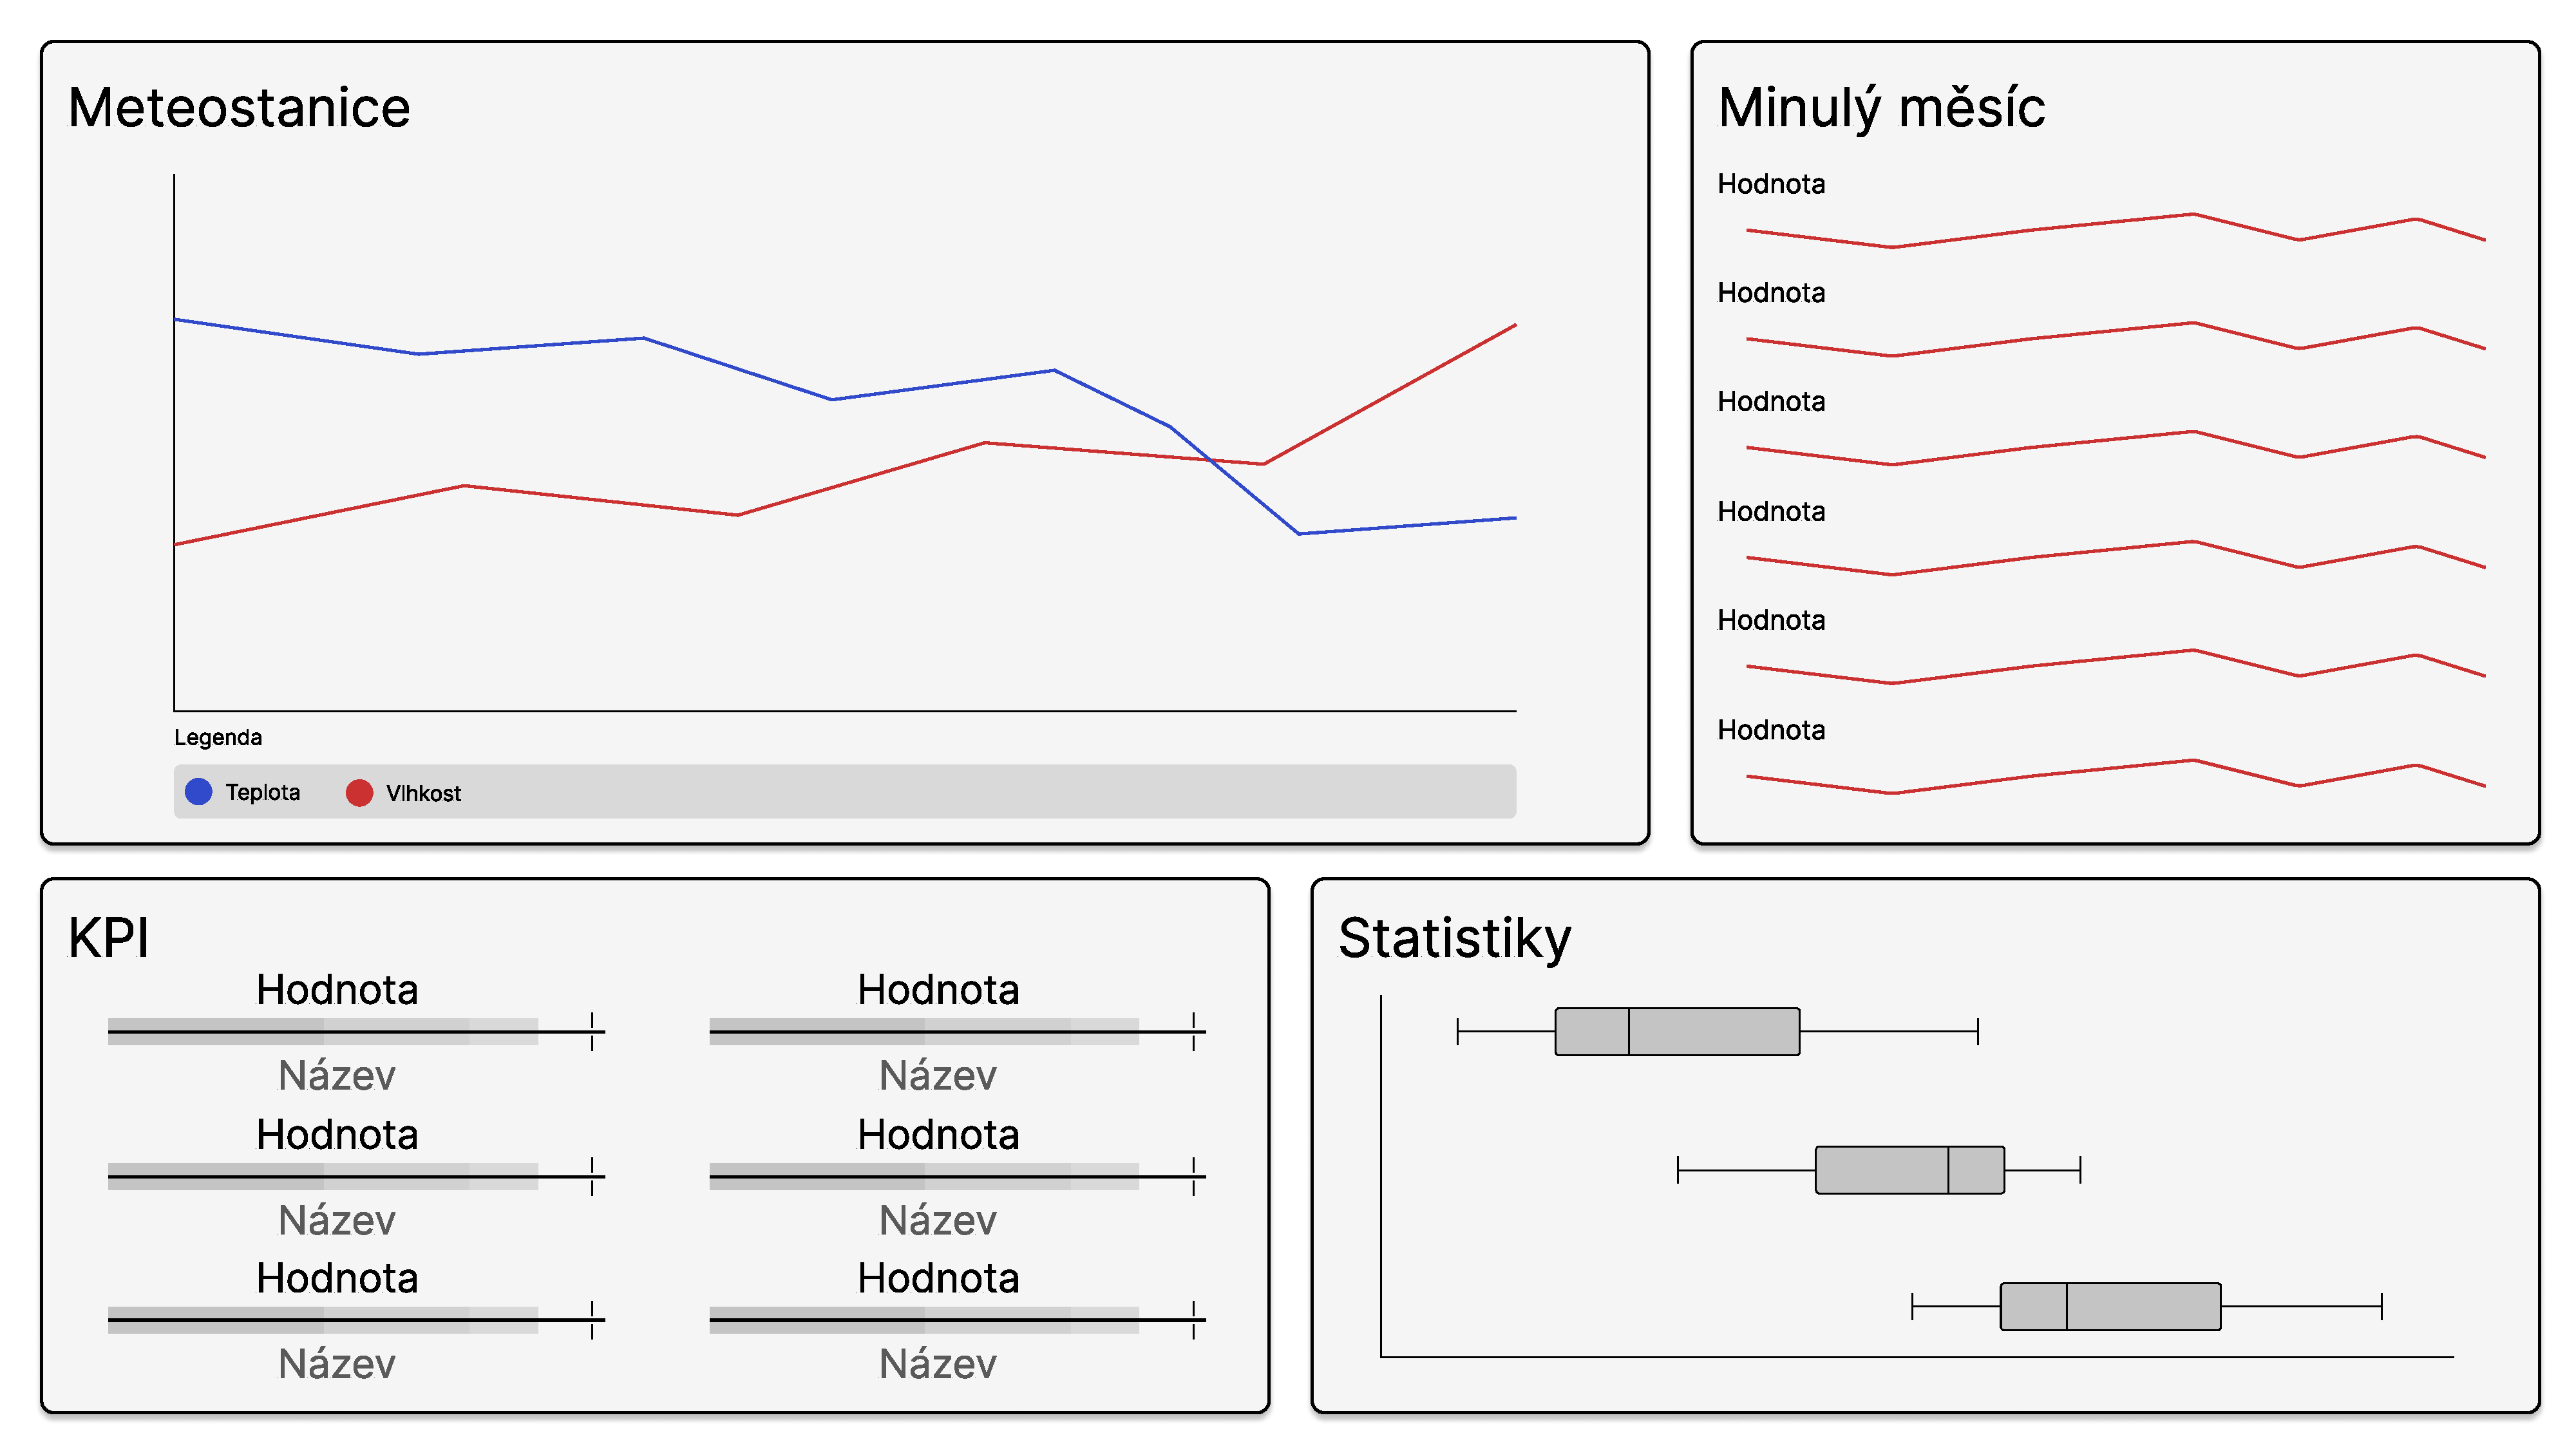
\includegraphics[width=0.9\textwidth]{obrazky-figures/view1.pdf}
\end{center}
\caption{Navrhované zobrazení}
\end{figure}

Toto navrhované zobrazení nabízí způsob, jak uživateli zobrazit aktuální stav zařízení s dostatečným porovnáním s historií tak, aby bylo na jeho základě možné vyhodnotit aktuální stav. Podobným způsobem s ohledem na problémy, které přináší zobrazení více zařízení v jednom pohledu, by bylo možné vyřešit i srovnání dvou senzorů.

\section{Zpřístupnění dat}

Ke komunikaci mezi databázovým systémem a aplikací zobrazující data je zapotřebí vytvořit dedikovanou vrstvu. Na cloudovém řešení připadá v úvahu využít takzvaných \uv{serverless} funkcí. Příkladem těchto funkcí jsou AWS Lambdy. Druhou možností je implementace aplikačního serveru, který bude tato data zpřístupňovat. 

V tomto konkrétním případě přichází v úvahu implementovat vlastní aplikační server, který bude v případě nutnosti možné jednoduše spustit jak na lokálním stroji tak na cloudovém řešení. Tato aplikace musí zpřístupňovat jak možnosti výběrů dat z databázového systému tak ukládat data ze zařízeních samotných.

I přes to, že data jsou přenášena pomocí MQTT bude aplikace zpracovávat pouze předpřipravená data v již dekódovaném formátu. Dekódování mohou provádět brány zmíněné v kapitole 1, cloudová řešení jako the thing stack, nebo jiné mikroslužby. Díky tomu bude možné použít aplikaci ve více případech než kdyby přijímala data ve formátu MQTT. Zároveň se sníží komplexita celé aplikace. Stejný přístup bude zachován i v případě autentifikace a autorizace.

I z důvodu jednoduché integrace byla při návrhu zvolena architektura REST. Kromě koncových bodů pro uložení dat bude aplikace poskytovat koncové body reprezentující výběry. Tyto koncové body musí umožnit výběr dat nejen na základě zadaného časového období, ale také zvoleného typu agregace a doby po kterou se na tato agregace provést. Tyto body nebudou dostačující pro všechny operace, které mohou vyžadovat vizualizace. Příkladem této operace může být výběr časových momentů, ve kterých se změní hodnota parametru.

\begin{figure}[H]
\label{question4}
\begin{center}
    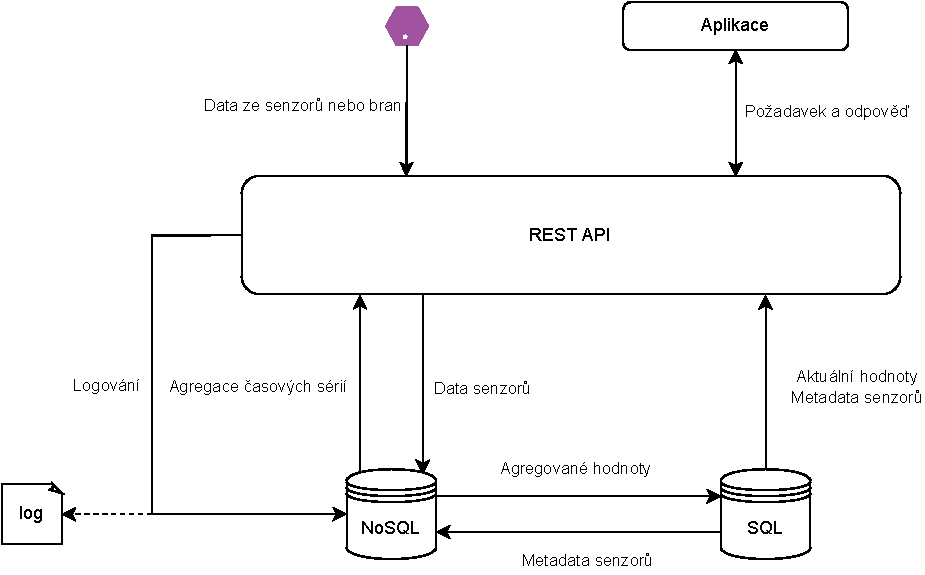
\includegraphics[width=0.9\textwidth]{obrazky-figures/layerArchitecture.pdf}
\end{center}
\caption{Navrhovaná architektura řešení}
\end{figure}

Praktickým řešením je vytvořit koncový bod pro každou další operaci, kterou bude nutné provádět. Tyto operace mohou odpovídat efektivním dotazům. O použití koncových bodů je praktické dělat záznam,díky kterému je možné vyhodnotit jeho využití, nebo útoky na něj. Tyto záznamy je možné ukládat jak do relačního tak do NoSQL databázového systému. I samotné záznamy tvoří svým způsobem časové série, protože přibývají a mění svoji důležitost s ohledem na čas.


\chapter{Implementace}
\label{chapter_implemenatation}
Po provedení návrhu je nutné zvolit řešení, jeho konkrétní implementační detaily a v neposlední řadě provést jeho realizaci. Tato sekce popisuje všechny části implementace v pořadí, ve kterém byly při řešení prováděny.

Všechny části řešení jsou implementovány v jazyce TypeScript. Tento jazyk byl zvolen díky transpilaci do JavaScriptu, která poskytuje možnost použít stejný jazyk jak pro frontend tak backend a částečně také kvůli stejnému použití firmou Logimic. 
\section{Výběr databázového systému}
Výběr databázového systému byl primárně zaměřen na systém, který bude umožňovat ukládání a zpracování dat ze senzorů. Zbylá data zůstávají uloženy v relačním databázovém systému PostgreSQL. Při výběru byly testovány systémy zmíněné v ref 2 na základě následujících metrik:
\begin{itemize}
\item prostředí - určuje, zdali je databázový systém možné jednoduše využít jak v cloudu tak na lokálních instancích bez výrazných omezení,
\item využití - k čemu je možné využít daný databázový systém, například zdali je určený pouze k ukládání časových sérii, nebo je možné ukládat i jiná data,
\item poskytované operace - určuje, zda databázový systém poskytuje operace, nebo dotazovací jazyk, který umožňuje efektivní práci s časovými sériemi,
\item výkon operací - rychlost provádění operací,
\item efektivita uložení - velikost uložených dat a režie.
\end{itemize}
Po stanovení těchto požadavků se projevil dosavadní databázový systém DynamoDB jako nepraktický. I přes to, že poskytuje možnost velmi rychlého zápisu a čtení konkrétní položky libovolné struktury, nepodporuje žádné speciální operace. Tento fakt se projevil v již existujících zobrazeních, kde způsobily nepříjemné čekání.

Složitější bylo srovnání u databázových systémů InfluxDB a MongoDB. Na první pohled poskytují oba systémy velmi podobné výhody. Největším rozdílem je to, že InfluxDB je více specializované na práci s časovými sériemi než MongoDB.

Aby bylo možné rozhodnout, který databázový systém je vhodnější pro využití v této konkrétní situaci bylo nutné využít posledních dvou metrik. Za tímto účelem byl vytvořen jednoduchý program, který testuje rychlosti vložení a čtení dat a provádění agregací. 

K testování byla vybrána data tradičně ukládaná firmou Logimic. Použití syntetických dat by mohlo negativním způsobem ovlivnit výsledky testování a vést k výběru méně vhodného řešení. V průběhu testování byl měřen čas jak jednotlivých operací tak celkového trvání celé sady. Díky tomu bylo možné srovnat jak celkový výkon tak trvání operací, které se budou často opakovat.

Srovnání velikosti bylo provedené velmi jednoduchým způsobem. Data byla vložena do obou systémů. Následně byla srovnána celková velikost na disku spotřebována k uložení dat. Pro referenci, zdali se přechod doopravdy vyplatí byly okrajově testovány i už používané systémy DynamoDB a PostgreSQL.

Obrázky a popis výsledků benchmarku

Nakonec byl zvolen databázový systém InfluxDB. Není sice plnou náhradou DynamoDB, ale z vybraných systémů se jeví jako nejpraktičtější pro jeho zamýšlené využití v této konkrétní situaci. V případě nedostatku výkonu v budoucnosti by bylo možné využít databázový systém MongoDB pro jako úložiště optimalizované pro rychlé čtení. Systém DynamoDB je v tomto ohledu sice rychlejší, ale problémem zůstává jeho závislost na cloudovém řešení AWS.

\section{Implementace vstvy zpřístupňující data}
Jak již bylo zmíněno v návrhu je praktické vytvořit vstvu, která bude oddělovat aplikaci zobrazující data. Pro implementaci byl zvolen webový aplikační rámec Express.js\footnote{Aplikační server Express.js: \url{https://github.com/expressjs/express}}. Express.js prezentuje možnost vytvořit rychlý a robustní aplikaci velmi jednoduchým způsobem. Díky jeho popularitě také existuje řada rozšíření, které je možné při implementaci použít. 

Při prvotním testování tohoto řešení byl detekován nárůst zdrojů potřebných k obsloužení funkcí na straně AWS. Kvůli tomuto faktu se vývoj této aplikace nakonec rozdělil na následující dva proudy: lokální API je reprezentováno aplikačním serverem založeným na rámci Express.js a AWS Lambdy.

Tento fakt byl jeden z důvodů, který vedl na implementaci nezávislé vrstvy, která bude zjednodušovat přístup k datům v databázi a bude možné ji využít v případě obou řešení. Díky tomu se omezí kód, který je nutné duplikovat mezi aplikacemi. Tato vrstva je založená na referenčním klientu pro InfluxDB\footnote{InfluxDB klient pro JavaScript: \url{https://github.com/influxdata/influxdb-client-js}}.

Na strukturu vstupních dat jsou kladeny velmi malé nároky. Vstupní struktura musí obsahovat název měření, ke kterému patří, nejčastěji reprezentováno pomocí identifikátor senzoru, a následně vlastní data. Při ukládání dat mohou být určité položky označeny za metadata, což umožní rychlejší filtrování na jejich základě.

\subsection{Lokální API}
Aplikační server Express.js byl doplněn dalšími nástroji, které zjednudušují vývoj a zajišťují škálovatelnost řešení. Mezi nejdůležitější z použitých nástrojů patří balíček pro vkládání závislostí typedi\footnote{Nástroj typedi: \url{https://github.com/typestack/typedi}} a nástroj zjednodušující vytváření REST aplikací tsoa\footnote{Nástroj tsoa: \url{https://github.com/lukeautry/tsoa}}.

Díky nástroji tsoa je možné rychle a přehledně vytvářet řadiče, anglicky \uv{controller}. Při použití dostupných dekorátorů v každém řadiči je možné vygenerovat jak část potřebného směrovač, anglicky \uv{router} tak specifikaci samotného API v podobě OpenAPI\footnote{Specifikace OpenAPI \url{https://swagger.io/specification/}} specifikace. 

Další výhodou této kombinace je možnost použití takzvaných \uv{middlewares}, které umožňují vykonávat logiku mimo kód obsluhující konkrétní koncový bod. Z praktického pohledu je možné middlewares srovnat například s aspekty v jiných programovacích jazycích. Při implementaci se nabízí jich využít například pro kontrolu autentizačního tokenu. 
%todo obrázek

Vstupní požadavek je obsloužen nejdříve pomocí middleware, který zkontroluje jeho platnost a až následně, pokud bude token platný bude řízení předáno obslužnému kódu koncového bodu. Tímto způsobem je možné vyřešit i ukládání historie použití.

I přes to, že data historie nepřipomínají data ze senzorů je praktické je uložit do systému InfluxDB. Kvůli limitacím ukládání je praktické pozměnit formát ukládaných dat. V některých případech může být ukládaná struktura vysoce zanořená, tato situace nastává například v momentu, kdy selže obshluha koncového bodu. Z pohledu následující analýzy chyby může být praktické uložit celý vstupní požadavek a další informace.

Pro následného vyhledávání jsou zanořené struktury problematické. Databázový systém jako takový nepodporuje jejich ukládání a je nutné je buď převést na strukturu, která není zanořená, nebo uložit data určená k vyhledávání duplicitně. Vytvořená vrstva poskytuje obě dvě možnosti, ale při implementaci byla využita možnost druhá. Tato možnost sice duplikuje data, ale je jednoduší ji integrovat do již existujícího systému.

Pro každou logickou část je v aplikaci vytvořen řadič, který tuto část zpravuje. Díky nástroji tsoa je částečně vyřešen i problém validace vstupních dat, jelikož jeho správné využití zajistí alespoň částečnou validaci a sanitizaci těchto dat na základě použitých typových definic jazyka TypeScript. Složitější validaci je nutné vykonat vlastní logikou například v již zmíněných middlewares.

Jedním z požadavků při vytváření aplikace byla dokumentace poskytovaného API. Jako řešení byla zvolena již zmíněná specifikace OpenAPI, kterou je možné generovat z kombinace dekorátorů a komentářů u použitých datových typů a vytvořených koncových bodů. 

Implementace tohoto požadavku se nakonec projevila jako velice výhodná. Ze vzniklé OpenAPI specifikace je možné generovat artefakty pro použití ve frontendové aplikaci. Pro toto generování byl zvolen nástroj \emph{ng-openapi-gen}\footnote{Nástroj ng-openapi-gen \url{https://github.com/cyclosproject/ng-openapi-gen}}, který generuje jak ekvivalenty použitých datových typů tak Angular služby. Díky tomu je možné odstínit frontend od implementačních detailů samotného API bez nutnosti ručně udržovat tuto vrstvu.

\subsection{Cloud AWS}
Na straně cloudu je situace podobná. Bohužel zde není možné použít nástroj tsoa a musí se proto zvolit vhodné alternativní řešení. I přes to, že je možné vytvářet a nasazovat jednotlivé lambdy přímo, často bývá lepší využít nástrojů, které proces zjednodušují. 

Ve firmě Logimic se používá nástroj serverless. Tento nástroj se postará jak o nasazení tak o zabalení více zdrojových souborů nástrojem webpack a ostatní konfiguraci, kterou jsou například oprávnění výsledné lambdy.

Aby bylo možné využívat vygenerované API artefakty i pro cloudové řešení je nutné synchronizovat cesty koncových bodů a jejich chování. Za tímto účelem je nutné ručně nastavit stejné cesty koncových bodů.

Lepší situace je v případě validace, kde je možné velkou část vyřešit pomocí nástrojů pro validaci. Jedním z těchto nástrojů je i \emph{ajv}, který poskytuje možnost provádět validaci i na základě JSON schémat\footnote{Zvolená verze JSON schémat \url{https://json-schema.org/draft-07/json-schema-release-notes.html}}. I v tomto případě se ukázala již existující specifikace OpenAPI jako výhodná. Díky ní je možné tyto schémata vygenerovat.

Stejně jako u generování artefaktů pro frontend je i v tomto řešení stejná nevýhoda. Pro plnou funkčnost je nutné udržovat jak lokální API, které je zdrojem generovaných JSON schémat.

\section{Implementace zobrazení}
Implementované pohledy a komponenty byly vytvořeny za pomocí rámce Angular. Pro další zjednodušení vývoje byly použity i nástroje \emph{PrimeNG}, který obsahuje sadu základních komponentů a \emph{PrimeFlex} pro zjednodušení pozicování elementů na stránce.

Tento výběr omezil možnost využití balíčku carbon charts, který vyžaduje použití balíčku bootstrap. Místo něj byla využita kombinace balíčků ngx-charts, vlastních vizualizací a rozšíření na něm založených a ApexCharts\footnote{ApexCharts \url{https://apexcharts.com/}} pro vizualizace, které nejsou ngx-charts dostupné.

Za pomocí těchto nástrojů a vygenerovaných komponentů popsaných v předchozí kapitole byl vytvořen navrhovaný pohled. Již při jeho implementaci bylo jasné, že bude nutné jej rozšířit o určité funkce. Příkladem těchto rozšíření je zobrazení statických informací jako je například aktuální verze software na zařízení, nebo datum posledního měření.

Další podstatnou částí, která v návrhu chyběla bylo ovládání zobrazení. Nakonec bylo zvoleno jednoduché ovládání, které uživateli umožňuje určit období a položky zvoleného zařízení, které mají být zobrazeny v hlavní části dashboardu. Po zobrazení dat je také možné využít sparkline umístěné pod grafem pro podrobnější zobrazení menšího časového období. 

I sparkline zobrazující trend byly rozšířeny. Nyní dovolují zobrazovat a skrývat uživatelem nastavené limity. Tato vlastnost sice poněkud komplikuje původní záměr tohoto typu vizualizace, ale na druhou stranu zvyšuje srovnávací schopnosti uživatele.

Stejné zobrazení poskytuje i možnost zobrazit jiné zařízení stejného typu. V tomto případě se pro obě zařízení zobrazí stejné metriky obou zařízení v úvodním grafu. I vzhled sparkline se změní. Při výběru dalšího zařízení se přidá druhá linie, které reprezentuje jeho hodnotu. Poslední zobrazení, které reaguje na výběr zařízení k srovnání jsou odrážkové grafy, kde je hodnota druhého zvoleného zařízení zobrazena pomocí ukazatele předchozí hodnoty. Krabicové grafy nereagují na volbu dalšího zařízení žádným způsobem.

Zařízení, které nejsou stejného typu by neměla být systémem srovnávána. Tato zařízení mohou mít například výstupy, které neměří stejné veličiny, nebo takové veličiny, které by byly závislé na veličinách právě zobrazeného zařízení. Problematické je i určit, zdali je možné srovnat dvě zařízení, které měří shodné veličiny. Například teplotu mohou měřit 2 různá zařízení s velmi rozdílnou přesností. 

Druhý vytvořený pohled je v mnoha pohledech velmi podobný tomu prvnímu. jeho hlavním prvkem je také spojnicový graf. Oproti předchozímu pohledu, ale nepřiřazuje velkou hodnotu statistickým zobrazením, žádným způsobem nezobrazuje statické, nebo ne často měnící se data a poskytuje omezenější ovládání. Na druhou stranu dává větší prioritu zobrazení dostupnosti zařízení.

Tento pohled byl navržen jako jednoduší verze zobrazení, kterou bude schopen využít i nezkušený uživatel, pro kterého by mohly být některé vizualizace velmi složité, nebo netradiční. Při tvorbě aplikace může být využito obou pohledů například pomocí uživatelského nastavení, kde by uživatel zvolil, který pohled chce zobrazit.

Oba dva tyto pohledy jsou více zaměřené na numerické než kategorické hodnoty. V praxi jsou ale časté případy, kdy je nutné zobrazit i kategorická data. Při spolupráci s firmou Logimic nastala přesně tato situace a zákazník vyžadoval pohled, respektive jeho část, která bude více přizpůsobená tomuto použití. 

V tomto případě se jednalo o zobrazení součtu počtů daných stavů v aktuálním dni, v každé hodině vybraného dne a každého dne vybraného týdne. Po konzultaci se zákazníkem byl za tímto účelem vybrán sloupcový graf, který dokáže tato data zobrazit zákazníkovi přívětivým způsobem. 

V případě součtu počtu stavů v aktuálním dni bylo hlavním účelem vizuálně zobrazit rozložení hodnot jednotlivých tříd. V původním návrhu měl k tomuto účelu sloužit kruhový diagram. V průběhu vývoje byl rychle vyměněn za horizontální sloupcový graf o jednom sloupci, který zobrazuje jak hodnoty samotných tříd, pomocí \uv{naskládání} dílčích sloupečků na sebe tak celkový součet hodnot všech tříd pomocí výšky celého sloupce. 

Tento přístup se postupně rozšířil na ostatní vizualizace, a to hlavně kvůli tomu, že představuje jednoduchý, efektivní a pro zákazníka přívětivý způsob zobrazení. Zbylé dvě vizualizace využívají vertikálních sloupcových grafů. V obou vizualizacích jsou zobrazeny i dny, nebo hodiny, které neobsahují žádné hodnoty. Toto rozhodnutí zlepšuje estetickou stránku vizualizace a může umožnit uživateli rychleji vyhodnotit zobrazená data. 

Původní komponent pro sloupcový graf neposkytoval možnost dočasně zrušit zobrazení jednotlivých tříd. Tato funkcionalita byla přidána jednoduchým způsobem. Po kliknutím na legendu odpovídající třídy se text legendy přeškrtne a hodnota se skryje.

I přes to, že byl tento pohled původně implementován na základě požadavku cílového zákazníka bylo přidáno ovládání a možnost nastavit počáteční hodnoty vizualizací. Díky tomu je možné vizualizaci použít i v pro jiné zákazníky, kteří budou mít podobný požadavek a to bez nutnosti editovat již vytvořené komponenty. Přidané ovládání poskytuje možnost nejen nastavit období ve kterém se mají zobrazit jednotlivé vzorky tak agregaci, která má být vykonána.

Kromě těchto požadavků měl výsledný pohled zobrazovat i součet počtů všech tříd ve třech časových úsecích: dnes, posledních 7 dní a posledních 30 dní. K zobrazení těchto dat nebyla využita žádná složitá vizualizace ale pouze jednoduchý text s názvem časového období a samotnou hodnotou.

Kromě samotných pohledů byly vytvořeny i komponenty, které v nich byly využity. Některé z těchto komponentů byly založeny na již existujících komponentech a jiné na rámci d3.js.

Prvním vytvořeným komponentem byl bullet chart, který není implementován v rámci ngx-charts. Pro jeho implementaci se zvolila strategie rozšíření již existujícího grafu, která zaručí vysokou vizuální podobnost k vizualizacím, které rámec již poskytuje. Tento přístup je také doporučují vývojáři balíčku.

Implementace byla založena na vizualizaci, kterou vývojáři rámce nazvali lineární budík, původním názvem \uv{linear gauge}. Tento graf je dobrým základem pro graf typu bullet, protože s ním sdílí velké množství rysů. Obě dvě vizualice jsou horizontální, zobrazují aktuální hodnotu pomocí sloupečku a druhou pomocí přerušené vertikální čáry. 

V implementaci je tedy nutné přidat popisky a sloupce, které budou sloužit k zobrazení jednotlivých prahů. Původní vizualizace má také jednu velmi nepraktickou vlastnost a to tu, že se při svém zobrazení snaží vyplnit dostupný prostor automatickým zvětšením velikosti textu. Takto zvětšený text nepůsobí dobře s ohledem k nadpisům, jelikož může velikostí. Výsledný komponent poskytuje možnost zapnout původní chování, nebo nastavit očekávanou velikost textu.

Druhým vytvořeným komponentem je speciální vizualizace určená k zobrazení změny stavu primárně kategorického atributu. Každému období se stejnou hodnotou atributu ve vizualizaci odpovídá obdélník, jehož šířka odpovídá procentuálnímu podílu tohoto období na celkovém zvoleném období. V případě, že je obdélník dostatečně veliký je v něm zobrazena aktuální hodnota. Při jeho zmenšování dochází ke snížení počtu zobrazených písmen. Každé zobrazené hodnotě je také přiřazena barva.

Tato kombinace dovoluje uživateli rychle vyhodnotit stav zařízení. Toto zobrazení ale není ideální pro použití v případech, kdy se hodnoty rychle mění na relativně dlouhém časovém období. Krátké změny mohou být zobrazeny příliš úzkými obdélníky, které uživatel neuvidí. 

Tento komponent byl plně implementován pomocí d3.js. Díky tomu je její velikost minimální a je možné ji použít v jakémkoli projektu prakticky bez přidání dalších závislostí. Při implementaci byl kladen důraz i na responzivitu samotné komponenty. Vizualizace se proto snaží využít co nejvíce prostoru, ve kterém se nachází.

Zbylé vytvořené komponenty představují spíše rozšíření komponent z již existujících balíčků takovým způsobem, aby byla zjednodušena jejich integrace do nových systémů. Některé z nich poskytují zvýšení abstrakce, zatímco jiné přidávají funkcionalitu, která v originálních komponentech chyběla.

\chapter{Testování}
Implementované části je vždy nutné nějakým způsobem otestovat. V případě vrstvy, která pracuje s databází a API je testování relativně jednoduché. Situace je výrazně horší u testování jednotlivých pohledů a vizualizací. 

U grafických prvků je nutné zajistit nejen jejich správnou funkčnost, ale také to, zdali odpovídají požadavkům uživatele a jestli je jejich použití dostatečně příjemné pro uživatele. 

\label{chapter_testing}
\chapter{Závěr}
V dnešní době se stále zvyšuje počet chytrých zařízení a s tím i množství dat, které je nutné získat, předzpracovat, uložit vyhodnotit a zobrazit uživateli. Tato semestrální práce se zaměřuje hlavně na způsoby efektivního uložení a zobrazení získaných dat z tradičních časových sérií.

V průběhu dalšího semestru budou navrženy a implementovány komponenty použitelné pro vytváření dashboardů. Tyto komponenty budou použity v ukázkové aplikaci tvořené dashboardy. K této aplikaci bude vytvořeno ještě jednoduché API, které bude prezentovat jednu z možností efektivního ukládání dat ze senzorů.

Určitým rozšířením by mohl být návrh vizualizací pro nestandardní typy senzorů jako je například záznam z kamery nebo optimalizace přenášených datových toků. Tyto datové toky mohou při velkém počtu senzorů představovat stálý provoz a může být optimální ukládat pouze agregovaná data.


  \fi
  
  % Kompilace po částech (viz výše, nutno odkomentovat)
  % Compilation piecewise (see above, it is necessary to uncomment it)
  %\subfile{projekt-01-uvod-introduction}
  % ...
  %\subfile{chapters/projekt-05-conclusion}


  % Pouzita literatura / Bibliography
  % ----------------------------------------------
\ifslovak
  \makeatletter
  \def\@openbib@code{\addcontentsline{toc}{chapter}{Literatúra}}
  \makeatother
  \bibliographystyle{bib-styles/Pysny/skplain}
\else
  \ifczech
    \makeatletter
    \def\@openbib@code{\addcontentsline{toc}{chapter}{Literatura}}
    \makeatother
    \bibliographystyle{bib-styles/Pysny/czplain}
  \else 
    \makeatletter
    \def\@openbib@code{\addcontentsline{toc}{chapter}{Bibliography}}
    \makeatother
    \bibliographystyle{bib-styles/Pysny/enplain}
  %  \bibliographystyle{alpha}
  \fi
\fi
  \begin{flushleft}
  \bibliography{projekt-20-literatura-bibliography}
  \end{flushleft}

  % vynechani stranky v oboustrannem rezimu
  % Skip the page in the two-sided mode
  \iftwoside
    \cleardoublepage
  \fi

  % Prilohy / Appendices
  % ---------------------------------------------
  \appendix
\ifczech
  \renewcommand{\appendixpagename}{Přílohy}
  \renewcommand{\appendixtocname}{Přílohy}
  \renewcommand{\appendixname}{Příloha}
\fi
\ifslovak
  \renewcommand{\appendixpagename}{Prílohy}
  \renewcommand{\appendixtocname}{Prílohy}
  \renewcommand{\appendixname}{Príloha}
\fi
%  \appendixpage

% vynechani stranky v oboustrannem rezimu
% Skip the page in the two-sided mode
%\iftwoside
%  \cleardoublepage
%\fi
  
\ifslovak
%  \section*{Zoznam príloh}
%  \addcontentsline{toc}{section}{Zoznam príloh}
\else
  \ifczech
%    \section*{Seznam příloh}
%    \addcontentsline{toc}{section}{Seznam příloh}
  \else
%    \section*{List of Appendices}
%    \addcontentsline{toc}{section}{List of Appendices}
  \fi
\fi
  \startcontents[chapters]
  \setlength{\parskip}{0pt} 
  % seznam příloh / list of appendices
  % \printcontents[chapters]{l}{0}{\setcounter{tocdepth}{2}}
  
  \ifODSAZ
    \setlength{\parskip}{0.5\bigskipamount}
  \else
    \setlength{\parskip}{0pt}
  \fi
  
  % vynechani stranky v oboustrannem rezimu
  \iftwoside
    \cleardoublepage
  \fi
  
  % Přílohy / Appendices
  \ifenglish
    \input{projekt-30-prilohy-appendices-en}
  \else
    \chapter{Obsah přiloženého paměťového média}
\begin{itemize}
    \item Tento dokument ve formátu pdf.
    \item source/README.md -- bližší popis repozitáře.
    \item source/backend -- backendová část práce.
    \begin{itemize}
        \item db-benchmark -- testování databází.
        \item InfluxDataBase --  vrstva zpřístupňující databází InfluxDB.
        \item express -- lokální API.
        \item influx-lambda -- AWS API.
    \end{itemize}
    \item source/frontend -- Angular aplikace.
    \begin{itemize}
        \item src/app/library -- vytvořená knihovna pohledů a vizualizací.
    \end{itemize}
\end{itemize}

  \fi
  
  % Kompilace po částech (viz výše, nutno odkomentovat)
  % Compilation piecewise (see above, it is necessary to uncomment it)
  %\subfile{projekt-30-prilohy-appendices}
  
\end{document}
